\documentclass[10pt]{article}

\usepackage[table,xcdraw]{xcolor}
\usepackage[utf8]{inputenc}
\usepackage{tabularx}
\usepackage{hyperref}
\usepackage{array}
\usepackage{graphicx} % Per inserire immagini (loghi)
\usepackage{geometry} % Per personalizzare i margini
\usepackage{fancyhdr} % Per gestire intestazioni e piè di pagina
\usepackage{tikz}
\usepackage{pgfplots}
\usepackage{pgf-pie}
\usepackage{ragged2e}
\usepackage{anyfontsize}
\usepackage{tabularx, etoolbox}
\usepackage{eso-pic} % Per aggiungere elementi grafici su tutte le pagine
\usepackage{float}
\usepackage{setspace}
\usepackage{longtable}

\RequirePackage{listings}
\RequirePackage[framemethod=TikZ]{mdframed}
\RequirePackage{xcolor}

% Minimal color setup
\definecolor{MLbg}{HTML}{F8F9FA}
\definecolor{MLborder}{HTML}{E6E6E6}
\definecolor{MLstring}{HTML}{D12F1B}
\definecolor{MLcomment}{HTML}{656565}
\definecolor{MLkeyword}{HTML}{703DAA}
\definecolor{MLidentifier}{HTML}{000000}

\mdfsetup{
    linewidth=1pt,
    linecolor=MLborder,
    backgroundcolor=MLbg,
    roundcorner=4pt,
    skipabove=\baselineskip,
    innertopmargin=6pt,
    innerbottommargin=6pt,
    innerleftmargin=6pt,
    innerrightmargin=6pt,
    skipbelow=\smallskipamount
}

\lstset{
    framesep=0pt,
    basicstyle=\ttfamily\small,
    columns=flexible,
    breaklines=true,
    tabsize=4,
    keepspaces=true,
    showstringspaces=false,
    commentstyle=\color{MLcomment},
    keywordstyle=\color{MLkeyword},
    stringstyle=\color{MLstring},
    numbers=left,
    numberstyle=\tiny\color{MLcomment},
    numbersep=1em,
    xleftmargin=0.8em,
    belowskip=-0.5\baselineskip
}

% Python definition
\lstdefinelanguage{Python}{
    morekeywords={and,as,assert,break,class,continue,def,del,elif,else,except,
        finally,for,from,global,if,import,in,is,lambda,nonlocal,not,or,pass,raise,
        return,try,while,with,yield},
    morecomment=[l]{\#},
    morestring=[b]"
}

% SQL definition
\lstdefinelanguage{SQL}{
    morekeywords={SELECT,FROM,WHERE,JOIN,INNER,LEFT,RIGHT,ON,GROUP,BY,HAVING,ORDER,
        INSERT,UPDATE,DELETE,CREATE,ALTER,DROP,INDEX,VALUES,INTO,PRIMARY,KEY,NULL},
    morecomment=[l]{--}
}

% JSON definition
\lstdefinelanguage{JSON}{
    morestring=[b]",
    morecomment=[l]{\#},
    literate=
     *{true}{{{\color{MLkeyword}true}}}{4}
        {false}{{{\color{MLkeyword}false}}}{5}
        {null}{{{\color{MLkeyword}null}}}{4}
}

\surroundwithmdframed{lstlisting}

\newcommand\version{0.1.4} %aggiunta versione come variabile
\newcommand{\myparagraph}[1]{\paragraph{#1}\mbox{}\\\vspace{0.4em}}


\graphicspath{{images/}}
%\graphicspath{{../images/}}

\setcounter{secnumdepth}{5}
\setcounter{tocdepth}{4}

%cambio misure della pagina
\geometry{a4paper,left=25mm,right=25mm,top=25mm,bottom=25mm}
\setlength{\parindent}{0pt}
\definecolor{colorePie}{HTML}{ebdfc7}
\pagestyle{fancy}
\fancyhf{}
\renewcommand{\headrulewidth}{0.4pt}
\lhead{
    \parbox[c]{1cm}{\includegraphics[width=1.1cm]{Sevenbitslogo.png}}
}
\rhead{\textcolor[HTML]{9e978a}{ SPECIFICA TECNICA v\version}
}
\setlength{\headheight}{25pt}
\cfoot{\thepage}

\renewcommand*\contentsname{Indice}
\renewcommand{\listfigurename}{Elenco delle figure}
\renewcommand{\listtablename}{Elenco delle tabelle}

\begin{document}

% Pagina del titolo
\begin{titlepage}
    \setcounter{page}{0}
    \centering
    % Inserisci il logo del gruppo (modifica il percorso dell'immagine)
    \includegraphics[width=7.2cm]{Sevenbitslogo.png} \\[2cm]

    % Titolo
     {\fontsize{40}{40}\bfseries Specifica Tecnica}\selectfont \\[3.9em]

    % Sottotitolo
    {\huge NearYou\\ \vspace{3mm }Smart custom advertising platform} \\[2.7em]

    % Email del gruppo
    {\large sevenbits.swe.unipd@gmail.com} \\[3em]

    % Spazio per il logo dell'università
    \hfill

    \AddToShipoutPictureBG{ % Imposta il triangolo con logo
        \ifnum\value{page}=0
        \begin{tikzpicture}[overlay]

            % Definisce un triangolo blu in basso a destra
            \fill[colorePie]
                (current page.south east) -- ++(-9cm,0) -- ++(9cm,9cm);

            % Inserisce il logo all'interno del triangolo
            \node[anchor=south east, xshift=-0.3cm, yshift=0.3cm] at (current page.south east) {
                \includegraphics[width=4.5cm]{LogoUnipd.png}
            };
        \end{tikzpicture}
        \fi
    }

\vfill % Aggiunge spazio verticale per centrare il contenuto
\end{titlepage}
\newpage
\clearpage
\setcounter{page}{1}

% Registro Modifiche
\begin{center}
 \textbf{Registro modifiche}\\   
\end{center}

\renewcommand{\arraystretch}{1.5}
\rowcolors{0}{gray!11}{white} % Aggiunge colore alternato alle righe

\begin{longtable}{|>{\centering\arraybackslash}m{1.5cm}|>{\centering\arraybackslash}m{2cm}|>{\centering\arraybackslash}m{2.5cm}|>{\centering\arraybackslash}m{2.5cm}|>{\centering\arraybackslash}m{5cm}|}
\hline
\textbf{Versione} & \textbf{Data} & \textbf{Autore} & \textbf{Verificatore} & \textbf{Descrizione}\\
\endhead
    \hline
    0.1.4 & 2025-03-16 & Riccardo Piva & Leonardo Trolese & Redazione generale macro sezioni documento \\ 
    \hline
    0.1.3 & 2025-03-05 & Alfredo Rubino & Manuel Gusella & Redazione sottosezione \hyperref[sec:strumenti]{Strumenti e Servizi} della sezione Tecnologie\\
    \hline
    0.1.2 & 2025-03-05 & Leonardo Trolese & Manuel Gusella & Conclusione redazione sottosezione \hyperref[sec:linguaggi]{Panoramica dei Linguaggi} della sezione Tecnologie\\
    \hline
    0.1.1 & 2025-03-02 & Leonardo Trolese & Manuel Gusella & Redazione sottosezione \hyperref[sec:linguaggi]{Panoramica dei Linguaggi} della sezione Tecnologie\\
    \hline
    0.1.0 & 2025-02-26 & Leonardo Trolese & Manuel Gusella & Inizio redazione del documento\\
    \hline
\end{longtable}
\rowcolors{0}{}{} % Riporta le righe alla colorazione originale

\newpage
\tableofcontents
\newpage
\listoffigures %elenco delle figure sarà da usare per ogni immagine
\newpage
\listoftables %lista delle tabelle presenti nel documento
\newpage
% \begin{justify}

\section{Introduzione}
\subsection{Scopo del documento}
Il presente documento si propone come una risorsa completa per la comprensione degli aspetti tecnici e progettuali della piattaforma "NearYou", dedicata alla 
creazione di soluzioni di advertising personalizzato tramite intelligenza artificiale. L’obiettivo principale è fornire una descrizione dettagliata dell’architettura 
implementativa e di deployment, illustrando le tecnologie adottate e le motivazioni alla base delle scelte progettuali.\\
Nel contesto dell'architettura implementativa, il documento analizza nel dettaglio i moduli principali del sistema, i design pattern utilizzati. Saranno inclusi 
diagrammi delle classi, e una spiegazione dettagliata dei design pattern utilizzati e delle motivazioni di queste scelte.\\
Gli obiettivi di questo documento sono: motivare le decisioni architetturali, fungere da guida per lo sviluppo della piattaforma, e garantire la piena tracciabilità e 
copertura dei requisiti definiti nel documento di \textit{Analisi dei Requisiti\_v1.0.0}.\\
In sintesi, il documento intende essere un punto di riferimento essenziale per tutti gli attori coinvolti nel ciclo di vita del progetto, offrendo una visione chiara e 
strutturata delle fondamenta tecniche che sorreggono NearYou e delle logiche che ne determinano il funzionamento.\\

\subsection{Glossario}
Con l'intento di evitare ambiguità interpretative del linguaggio utilizzato, viene fornito un Glossario che si occupa di esplicitare il significato dei termini che riguardano il contesto del Progetto$_G$. I termini presenti nel glossario sono contrassegnati con una \textit{G} a pedice : Termine$_G$.\\
I termini composti, oltre alla $_G$ a pedice, saranno uniti da un "-" come segue: termine-composto$_G$.\\
Le definizioni sono presenti nell'apposito documento \textit{Glossario\_v1.0.0.pdf}.

\subsection{Riferimenti}
\subsubsection{Riferimenti normativi}
\begin{itemize}
    \item[-] Regolamento del Progetto$_G$ didattico  \\
    \textcolor{blue}{\texttt{\url{https://www.math.unipd.it/~tullio/IS-1/2024/Dispense/PD1.pdf}}}\\ (Consultato: 2025-02-10).
    \item[-] Capitolato$_G$ C4 - NearYou - Smart custom advertising platform\\
    \textcolor{blue}{\texttt{\url{https://www.math.unipd.it/~tullio/IS-1/2024/Progetto/C4p.pdf}}}\\ (Consultato: 2025-02-10).
    \item[-] \textit{Norme\_di\_Progetto\_v1.0.0}
\end{itemize}

\subsubsection{Riferimenti informativi}
\begin{itemize}
    \item[-] \textit{Glossario\_v1.0.0}
    \item[-] \textit{Analisi\_dei\_Requisiti\_v1.0.0}
    \item[-] Analisi-dei-Requisiti$_G$ - SWE 2024-25\\
    \textcolor{blue}{\texttt{\url{https://www.math.unipd.it/\~tullio/IS-1/2024/Dispense/T05.pdf}}}\\ (Consultato: 2025-02-10).
    
    \item[-] Dependency Injection - SWE 2024-25\\    
    \textcolor{blue}{\texttt{\url{https://www.math.unipd.it/\~rcardin/swea/2022/Design\%20Pattern\%20Architetturali\%20-\%20Dependency\%20Injection.pdf}}}\\ (Consultato: 2025-02-26).
    
    \item[-] Design Pattern Creazionali - SWE 2024-25\\
    \textcolor{blue}{\texttt{\url{https://www.math.unipd.it/\~rcardin/swea/2022/Design\%20Pattern\%20Creazionali.pdf}}}\\ (Consultato: 2025-02-26).
    
    \item[-] Design Pattern Strutturali - SWE 2024-25\\
    \textcolor{blue}{\url{https://www.math.unipd.it/\~rcardin/swea/2022/Design\%20Pattern\%20Strutturali.pdf}}\\ (Consultato: 2025-02-26).
    
    \item[-] Software Architecture Patterns - SWE 2024-25\\
    \textcolor{blue}{\url{https://www.math.unipd.it/\~rcardin/swea/2022/Software\%20Architecture\%20Patterns.pdf}}\\ (Consultato: 2025-02-26).
    
    \item[-] Verbali Interni
    \item[-] Verbali Esterni
\end{itemize}


\section{Tecnologie}
Questa sezione descrive le tecnologie utilizzate per lo sviluppo del sistema NearYou, presentando una panoramica degli strumenti, dei linguaggi e dei servizi impiegati, con le motivazioni alla base delle scelte effettuate.

\subsection{Panoramica tecnologica}
Il sistema NearYou si basa su un'architettura a microservizi event-driven che utilizza diverse tecnologie integrate:

\begin{itemize}
    \item \textbf{Python}: Linguaggio principale per lo sviluppo dei componenti del sistema
    \item \textbf{Apache Kafka}: Sistema di messaggistica distribuito per la comunicazione tra componenti
    \item \textbf{Apache Flink}: Framework di elaborazione dati in tempo reale
    \item \textbf{ClickHouse}: Database colonnare ad alte prestazioni
    \item \textbf{Grafana}: Piattaforma di visualizzazione dei dati in tempo reale
    \item \textbf{Docker}: Sistema di containerizzazione per il deployment
\end{itemize}

\subsection{Linguaggi di programmazione}
\label{sec:linguaggi}

\subsubsection{Python}
Linguaggio di programmazione ad alto livello, interpretato e orientato agli oggetti, scelto per la sua leggibilità, la vasta libreria standard e l'ampio ecosistema di framework disponibili, particolarmente adatto allo sviluppo rapido di applicazioni.

\paragraph{Specifiche}
\begin{itemize}
    \item \textbf{Versione}: 3.12.2
    \item \textbf{Documentazione}: \textcolor{blue}{\url{https://docs.python.org/}} (Consultato: 2025-03-02)
\end{itemize}

\paragraph{Ruolo nel progetto}
Nel contesto di NearYou, Python viene impiegato per:
\begin{itemize}
    \item[-] Sviluppo del simulatore di spostamenti utente
    \item[-] Implementazione della logica di elaborazione dati
    \item[-] Interazione con i servizi esterni e le API
    \item[-] Gestione della persistenza dei dati
    \item[-] Applicazione degli algoritmi di selezione dei POI rilevanti
\end{itemize}

\paragraph{Dipendenze}
\begin{itemize}
    \item[-] \textbf{ClickHouse Connect}:
    \begin{itemize}
        \item \textbf{Descrizione}: Libreria client per l'interazione con il database ClickHouse, permettendo operazioni di query e gestione dei dati.
        \item \textbf{Versione}: 0.6.8
        \item \textbf{Documentazione}: \textcolor{blue}{\url{https://clickhouse.com/docs/integrations/python}} (Consultato: 2025-03-02)
    \end{itemize}
    
    \item[-] \textbf{PyFlink}:
    \begin{itemize}
        \item \textbf{Descrizione}: API Python di Apache Flink per l'elaborazione di flussi di dati distribuiti, sia in modalità batch che streaming.
        \item \textbf{Verione}: 1.18.1
        \item \textbf{Documentazione}: \textcolor{blue}{\url{https://pyflink.readthedocs.io/en/main/getting_started/index.html}} (Consultato: 2025-03-02)
    \end{itemize}
    
    \item[-] \textbf{LangChain}:
    \begin{itemize}
        \item \textbf{Descrizione}: Framework per lo sviluppo di applicazioni basate su modelli linguistici, consentendo di orchestrare prompt e integrare fonti di dati esterne.
        \item \textbf{Versione}: 0.1.12
        \item \textbf{Documentazione}: \textcolor{blue}{\url{https://python.langchain.com/docs/introduction/}} (Consultato: 2025-03-02)
    \end{itemize}
    
    \item[-] \textbf{Groq}:
    \begin{itemize}
        \item \textbf{Descrizione}: Client Python per l'API Groq, utilizzato per la generazione di contenuti tramite LLM.
        \item \textbf{Versione}: 0.4.2
        \item \textbf{Documentazione}: \textcolor{blue}{\url{https://console.groq.com/docs/libraries}} (Consultato: 2025-03-02)
    \end{itemize}
    
    \item[-] \textbf{Confluent Kafka}:
    \begin{itemize}
        \item \textbf{Descrizione}: Libreria per l'interazione con Apache Kafka, utilizzata per la pubblicazione e sottoscrizione di messaggi.
        \item \textbf{Versione}: 2.8.0
        \item \textbf{Documentazione}: \textcolor{blue}{\url{https://docs.confluent.io/kafka/overview.html}} (Consultato: 2025-03-02)
    \end{itemize}
    
    \item[-] \textbf{GeoPy}:
    \begin{itemize}
        \item \textbf{Descrizione}: Libreria per operazioni geospaziali e calcolo delle distanze.
        \item \textbf{Versione}: 2.4.1
        \item \textbf{Documentazione}: \textcolor{blue}{\url{https://geopy.readthedocs.io/en/stable/index.html}} (Consultato: 2025-03-02)
    \end{itemize}
    
    \item[-] \textbf{OSMnx}:
    \begin{itemize}
        \item \textbf{Descrizione}: Libreria per scaricare e analizzare reti stradali da OpenStreetMap, utilizzata per simulare percorsi realistici.
        \item \textbf{Versione}: 1.9.1
        \item \textbf{Documentazione}: \textcolor{blue}{\url{https://osmnx.readthedocs.io/en/stable/}} (Consultato: 2025-03-02)
    \end{itemize}
    
    \item[-] \textbf{Faker}:
    \begin{itemize}
        \item \textbf{Descrizione}: Libreria per la generazione di dati realistici per test.
        \item \textbf{Versione}: 24.1.0
        \item \textbf{Documentazione}: \textcolor{blue}{\url{https://faker.readthedocs.io/en/master/}} (Consultato: 2025-03-02)
    \end{itemize}
    
    \item[-] \textbf{Pylint}:
    \begin{itemize}
        \item \textbf{Descrizione}: Strumento di analisi statica del codice Python.
        \item \textbf{Versione}: 3.0.3
        \item \textbf{Documentazione}: \textcolor{blue}{\url{https://pylint.pycqa.org/en/latest/index.html}} (Consultato: 2025-03-03)
    \end{itemize}
    
    \item[-] \textbf{pytest}:
    \begin{itemize}
        \item \textbf{Descrizione}: Framework per test automatizzati.
        \item \textbf{Versione}: 7.4.3
        \item \textbf{Documentazione}: \textcolor{blue}{\url{https://docs.pytest.org/en/stable/}} (Consultato: 2025-03-03)
    \end{itemize}
\end{itemize}

\subsubsection{SQL}
Linguaggio standard per l'interrogazione e la manipolazione di database relazionali, utilizzato nel contesto di ClickHouse per definire lo schema del database e per interrogare i dati.

\paragraph{Specifiche}
\begin{itemize}
    \item \textbf{Dialetto}: ClickHouse SQL
    \item \textbf{Documentazione}: \textcolor{blue}{\url{https://clickhouse.com/docs/sql-reference}} (Consultato: 2025-03-05)
\end{itemize}

\paragraph{Ruolo nel progetto}
In NearYou, SQL viene utilizzato per:
\begin{itemize}
    \item[-] Definizione dello schema del database
    \item[-] Interrogazione dei dati per la visualizzazione
    \item[-] Creazione di query analitiche per l'identificazione delle relazioni spaziali
\end{itemize}

\subsubsection{Formati di interscambio dati}
\paragraph{YAML}
YAML è un formato di serializzazione dei dati human-readable basato sull'indentazione, utilizzato principalmente per file di configurazione.

\paragraph{Specifiche}
\begin{itemize}
    \item \textbf{Versione}: 1.2
    \item \textbf{Documentazione}: \textcolor{blue}{\url{https://yaml.org/spec/1.2.2/}} (Consultato: 2025-03-05)
\end{itemize}

\paragraph{Ruolo nel progetto}
\begin{itemize}
    \item[-] Configurazione dell'ambiente Docker
    \item[-] Workflow CI/CD
    \item[-] Configurazione dei servizi
\end{itemize}

\paragraph{JSON}
JSON è un formato di interscambio dati leggero e indipendente dal linguaggio, basato su coppie chiave-valore.

\paragraph{Specifiche}
\begin{itemize}
    \item \textbf{Versione}: 2.0
    \item \textbf{Documentazione}: \textcolor{blue}{\url{https://developer.mozilla.org/en-US/docs/Web/JavaScript/Reference/Global_Objects/JSON}} (Consultato: 2025-03-02)
\end{itemize}

\paragraph{Ruolo nel progetto}
\begin{itemize}
    \item[-] Serializzazione dei messaggi scambiati tra i componenti
    \item[-] Configurazione delle dashboard di visualizzazione
    \item[-] Comunicazione con i servizi API esterni
\end{itemize}

\subsection{Infrastruttura e servizi}
\label{sec:strumenti}

\subsubsection{Apache ZooKeeper}
Servizio di coordinamento distribuito che fornisce primitive per la gestione della configurazione, la sincronizzazione e la denominazione dei nodi in sistemi distribuiti.

\paragraph{Specifiche}
\begin{itemize}
    \item \textbf{Versione}: 7.6.0
    \item \textbf{Documentazione}: \textcolor{blue}{\url{https://zookeeper.apache.org/documentation.html}} (Consultato: 2025-03-05)
\end{itemize}

\paragraph{Ruolo nel progetto}
In NearYou, ZooKeeper è utilizzato per:
\begin{itemize}
    \item[-] Gestione dei broker Kafka e delle loro configurazioni
    \item[-] Monitoraggio dello stato dei nodi nel sistema distribuito
    \item[-] Coordinamento delle operazioni distribuite tra i componenti
    \item[-] Gestione delle elezioni dei leader per le partizioni Kafka
\end{itemize}

\subsubsection{Apache Kafka}
Sistema di messaggistica distribuita in grado di gestire flussi di dati in tempo reale, caratterizzato da elevata scalabilità, affidabilità e tolleranza ai guasti.

\paragraph{Specifiche}
\begin{itemize}
    \item \textbf{Versione}: 7.6.0
    \item \textbf{Documentazione}: \textcolor{blue}{\url{https://kafka.apache.org/documentation/}} (Consultato: 2025-03-05)
\end{itemize}

\paragraph{Ruolo nel progetto}
In NearYou, Kafka rappresenta il backbone della comunicazione tra componenti:
\begin{itemize}
    \item[-] Gestione del flusso di dati di posizione dagli utenti
    \item[-] Trasferimento dei messaggi pubblicitari generati
    \item[-] Garanzia di consegna delle informazioni anche in caso di guasti
    \item[-] Supporto al pattern event-driven dell'architettura
\end{itemize}

\subsubsection{Apache Flink}
Framework di elaborazione dati stream e batch distribuito, caratterizzato da bassa latenza, elevato throughput e gestione efficiente dello stato.

\paragraph{Specifiche}
\begin{itemize}
    \item \textbf{Versione}: 1.20.0
    \item \textbf{Documentazione}: \textcolor{blue}{\url{https://nightlies.apache.org/flink/flink-docs-stable/}} (Consultato: 2025-03-05)
\end{itemize}

\paragraph{Ruolo nel progetto}
In NearYou, Flink è utilizzato per:
\begin{itemize}
    \item[-] Elaborazione in tempo reale dei dati di posizione
    \item[-] Calcolo della prossimità tra utenti e punti di interesse tramite clickhouse
    \item[-] Orchestrazione del processo di generazione dei messaggi pubblicitari tramite LLM
    \item[-] Configurazione dei job per l'elaborazione dei dati 
\end{itemize}

\subsubsection{ClickHouse}
Database colonnare progettato per l'analisi OLAP (Online Analytical Processing) con prestazioni eccezionali su grandi volumi di dati.

\paragraph{Specifiche}
\begin{itemize}
    \item \textbf{Versione}: 24.10
    \item \textbf{Documentazione}: \textcolor{blue}{\url{https://clickhouse.com/docs/en/}} (Consultato: 2025-03-05)
\end{itemize}

\paragraph{Ruolo nel progetto}
In NearYou, ClickHouse è utilizzato per:
\begin{itemize}
    \item[-] Archiviazione dei dati di posizione degli utenti
    \item[-] Rilevamento della prossimità tra utenti e punti di interesse
    \item[-] Memorizzazione delle informazioni sui punti di interesse
    \item[-] Storicizzazione dei messaggi pubblicitari generati
    \item[-] Supporto alle query analitiche per la visualizzazione
\end{itemize}

\paragraph{Caratteristiche principali}
\begin{itemize}
    \item[-] Architettura colonnare per interrogazioni analitiche efficienti
    \item[-] Supporto a funzioni geospaziali per calcoli di distanza
    \item[-] Integrazione nativa con Kafka per l'ingestione di dati
    \item[-] Scalabilità orizzontale per gestire grandi volumi di dati
\end{itemize}

\subsubsection{Grafana}
Piattaforma open-source per la visualizzazione e il monitoraggio dei dati, con supporto per diverse fonti di dati e creazione di dashboard interattive.

\paragraph{Specifiche}
\begin{itemize}
    \item \textbf{Versione}: 11.5.2
    \item \textbf{Documentazione}: \textcolor{blue}{\url{https://grafana.com/docs/}} (Consultato: 2025-03-05)
\end{itemize}

\paragraph{Ruolo nel progetto}
In NearYou, Grafana è utilizzato per:
\begin{itemize}
    \item[-] Visualizzazione in tempo reale delle posizioni degli utenti
    \item[-] Rappresentazione dei punti di interesse sulla mappa
    \item[-] Monitoraggio dei messaggi pubblicitari generati
    \item[-] Creazione di dashboard interattive per l'analisi dei dati
\end{itemize}

\subsubsection{Docker}
Piattaforma di containerizzazione che consente di impacchettare applicazioni con le loro dipendenze in unità standardizzate chiamate container.

\paragraph{Specifiche}
\begin{itemize}
    \item \textbf{Versione}: 28.0.1
    \item \textbf{Documentazione}: \textcolor{blue}{\url{https://docs.docker.com/}} (Consultato: 2025-03-05)
\end{itemize}

\paragraph{Ruolo nel progetto}
In NearYou, Docker è utilizzato per:
\begin{itemize}
    \item[-] Containerizzazione dei diversi componenti del sistema
    \item[-] Creazione di un ambiente di sviluppo e deployment coerente
    \item[-] Semplificazione della distribuzione dell'applicazione
    \item[-] Isolamento dei servizi e gestione delle dipendenze
\end{itemize}

% \section{Tecnologie}
% Questa sezione descrive strumenti e tecnologie impiegate nello sviluppo del software del progetto NearYou.\\
% Saranno analizzate quindi le tecnologie utilizzate per lo sviluppo del software, le librerie e i framework utilizzati, e le motivazioni di queste scelte.

% \subsection{Panoramica dei linguaggi}
% \label{sec:linguaggi}
%     \subsubsection{Python}
%         Si tratta di un linguaggio di programmazione ad alto livello, interpretato e orientato agli oggetti, noto per la sua sintassi chiara e leggibile. Python dispone
%         anche di una vasta libreria standard ed è caratterizzato dalla grande quantità di framework disponibili.\\
%         \myparagraph{Versione}
%             3.12.2
%         \myparagraph{Documentazione}
%                  \textcolor{blue}{\url{https://docs.python.org/}} (Consultato: 2025-03-02)
%         \paragraph{Utilizzo operato nel progetto}
%             \begin{itemize}
%                 \item[-] Creazione dei sensori e simulazione degli spostamenti;
%                 \item[-] Generazione dei punti di interesse oggetto del messaggio pubblicitario;
%                 \item[-] Interazione con il database per la persistenza dei dati;
%                 \item[-] Interazione con l'LLM mediante API;
%                 \item[-] Logica di selezione dei punti di interesse rilevanti per l'utente;
%                 \item[-] Testing.
%             \end{itemize}
%         \paragraph{Dipendenze}
%             \begin{itemize}
%                 \item[-] ClickHouse Connect
%                     \begin{itemize}
%                         \item[.] Versione: 0.6.8
%                         \item[.] Documentazione: \textcolor{blue}{\url{https://clickhouse.com/docs/integrations/python}} (Consultato: 2025-03-02)
%                         \item[.] Descrizione: ClickHouse Connect è una libreria Python che consente di connettersi al database ClickHouse, eseguire query SQL 
%                         in modo veloce ed efficiente.
%                     \end{itemize}
%                 \item[-] PyFlink
%                     \begin{itemize}
%                         \item[.] Versione: 1.18.1
%                         \item[.] Documentazione: \textcolor{blue}{\url{https://pyflink.readthedocs.io/en/main/getting_started/index.html}} (Consultato: 2025-03-02)
%                         \item[.] Descrizione: PyFlink è l’API Python di Apache Flink, che permette di scrivere e gestire applicazioni per l'elaborazione di 
%                         flussi e batch di dati distribuiti in tempo reale, sfruttando la potenza e la scalabilità di Flink direttamente con Python.
%                     \end{itemize}
%                 \item[-] LangChain
%                     \begin{itemize}
%                         \item[.] Versione: 0.1.12
%                         \item[.] Documentazione: \textcolor{blue}{\url{https://python.langchain.com/docs/introduction/}} (Consultato: 2025-03-02)
%                         \item[.] Descrizione: LangChain è una libreria Python che semplifica la creazione di applicazioni basate su modelli linguistici, 
%                         consentendo di orchestrare prompt, gestire la memoria della conversazione e integrare fonti di dati esterne.
%                     \end{itemize}
%                 \item[-] Groq
%                     \begin{itemize}
%                         \item[.] Versione: 0.4.2
%                         \item[.] Documentazione: \textcolor{blue}{\url{https://console.groq.com/docs/libraries}} (Consultato: 2025-03-02)
%                         \item[.] Descrizione: Groq è una libreria Python che permette di interagire con modelli di linguaggio tramite API, facilitando la 
%                         generazione di testo, risposte conversazionali e completamenti.
%                     \end{itemize}
%                 \item[-] Confluent Kafka
%                     \begin{itemize}
%                         \item[.] Versione: 2.8.0
%                         \item[.] Documentazione: \textcolor{blue}{\url{https://docs.confluent.io/kafka/overview.html}} (Consultato: 2025-03-02)
%                         \item[.] Descrizione: Confluent Kafka è una libreria Python che semplifica l’interazione con Apache Kafka, permettendo di produrre, 
%                         consumare e gestire stream di dati in tempo reale, sfruttando la piattaforma Confluent.
%                     \end{itemize}
%                 \item[-] GeoPy
%                 \begin{itemize}
%                     \item[.] Versione: 2.4.1
%                     \item[.] Documentazione: \textcolor{blue}{\url{https://geopy.readthedocs.io/en/stable/index.html}} (Consultato: 2025-03-02)
%                     \item[.] Descrizione: GeoPy è una libreria Python che facilita la geocodifica, il calcolo delle distanze e l'interazione con servizi di localizzazione.
%                 \end{itemize}
%                 \item[-] OSMnx
%                     \begin{itemize}
%                         \item[.] Versione: 1.9.1
%                         \item[.] Documentazione: \textcolor{blue}{\url{https://osmnx.readthedocs.io/en/stable/}} (Consultato: 2025-03-02)
%                         \item[.] Descrizione: OSMnx è una libreria Python per scaricare, analizzare e visualizzare reti stradali e dati geografici da OpenStreetMap, 
%                         utile per creare grafi, calcolare percorsi e studiare l’urbanistica.
%                     \end{itemize}
%                 \item[-] Faker
%                     \begin{itemize}
%                         \item[.] Versione: 24.1.0
%                         \item[.] Documentazione: \textcolor{blue}{\url{https://faker.readthedocs.io/en/master/}} (Consultato: 2025-03-02)
%                         \item[.] Descrizione: Faker è una libreria Python che genera dati falsi realistici, come nomi, indirizzi, email o testi casuali, utile per test, 
%                         mock di database e prototipazione.
%                     \end{itemize}
%                 \item[-] Pylint
%                     \begin{itemize}
%                         \item[.] Versione: 3.0.3
%                         \item[.] Documentazione: \textcolor{blue}{\url{https://pylint.pycqa.org/en/latest/index.html}} (Consultato: 2025-03-03)
%                         \item[.] Pylint è uno strumento di analisi statica del codice Python per rilevare errori, violazioni di stile e migliorare la qualità del codice.
%                     \end{itemize}
%                 \item[-] pytest
%                     \begin{itemize}
%                         \item[.] Versione: 7.4.3
%                         \item[.] Documentazione: \textcolor{blue}{\url{https://docs.pytest.org/en/stable/}} (Consultato: 2025-03-03)
%                         \item[.] Descrizione: pytest è una libreria Python potente e flessibile che consente di scrivere ed eseguire test automatizzati, con funzionalità avanzate come 
%                         asserzioni intuitive, fixture e supporto per test parametrizzati.
%                     \end{itemize}
%             \end{itemize}

%     \subsubsection{SQL (Structured Query Language)}
%     Utilizzato per l'interazione con il database ClickHouse, un DBMS colonnare ad alte prestazioni, che supporta un sottoinsieme di SQL con estensioni specifiche.
%         \myparagraph{Versione}
%             24.10
%         \myparagraph{Documentazione}
%             \textcolor{blue}{\url{https://clickhouse.com/docs/sql-reference}} (Consultato: 2025-03-05)
%         \paragraph{Utilizzo operato nel progetto}
%             \begin{itemize}
%                 \item[-] Definizione schema del database;
%                 \item[-] Query per il recupero dei dati per la visualizzazione;
%                 \item[-] Query per il recupero dei dati per la generazione dei messaggi pubblicitari.
%             \end{itemize}

%     \subsubsection{YAML (YAML Ain't Markup Language)}
%     YAML è un linguaggio di serializzazione dei dati human-readable progettato per essere facilmente leggibile dall'uomo. La sua 
%     sintassi è basata sull'indentazione e ha una struttura chiave-valore. YAML è spesso usato in file di configurazione.
%         \myparagraph{Versione} 
%             1.2
%         \myparagraph{Documentazione}
%            \textcolor{blue}{\url{https://yaml.org/spec/1.2.2/}} (Consultato: 2025-03-05)
%         \paragraph{Utilizzo operato nel progetto}
%             \begin{itemize}
%                 \item[-] \textit{docker-compose.yml} per la configurazione dei servizi;
%                 \item[-] Workflow GitHub Actions per CI/CD;
%                 \item[-] File di configurazione per Grafana;
%                 \item[-] File di configurazione per i test.
%             \end{itemize}
%         \paragraph{Framework e tools correlati}
%             \begin{itemize}
%                 \item[-] Docker Compose;
%                 \item[-] GitHub Actions;
%                 \item[-] Grafana.
%             \end{itemize}

%     \subsubsection{JSON (JavaScript Object Notation)}
%     JSON è un formato di interscambio dati leggero, text-based e indipendente dal linguaggio, che utilizza una struttura di coppie 
%     chiave-valore e array. Progettato per essere facilmente leggibile sia dall'uomo che dalle macchine.
%         \myparagraph{Versione} 
%             2.0
%         \myparagraph{Documentazione}
%         \textcolor{blue}{\url{https://developer.mozilla.org/en-US/docs/Web/JavaScript/Reference/Global_Objects/JSON}} (Consultato: 2025-03-02)
%         \paragraph{Utilizzo operato nel progetto}
%             \begin{itemize}
%                 \item[-] Configurazione dashboard Grafana;
%                 \item[-] Invio e ricezione dati mediante il broker Kafka;
%                 \item[-] Risposta API del servizio Groq;
%             \end{itemize}
%         \paragraph{Framework e tools correlati}
%             \begin{itemize}
%                 \item[-] Groq;
%                 \item[-] Kafka;
%                 \item[-] Grafana.
%             \end{itemize}


% \subsection{Strumenti e servizi}
% \label{sec:strumenti}

%     \subsubsection{Docker}
%     Per lo sviluppo, il testing e il rilascio dell'applicativo sono stati usati dei container Docker, come suggerito dalla proponente, al fine di garantire ambienti di sviluppo e di test isolati, consistenti e riproducibili.\\
%     Docker è una piattaforma di containerizzazione che permette di eseguire applicazioni in ambienti isolati e riproducibili.
    
%     \myparagraph{Versione}  
%     28.0.1 %da controllare

%     \myparagraph{Documentazione}
%     \textcolor{blue}{\url{https://docs.docker.com/}} (Consultato: 2025-03-05)

%     \paragraph{Utilizzo nel progetto}
%     \begin{itemize}
%         \item[-] Creazione di container per il database, il backend e il servizio di elaborazione dati;
%         \item[-] Definizione di un ambiente standardizzato per il deployment.
%     \end{itemize}

%     \subsubsection{Grafana}
%     Grafana è una piattaforma open-source per la visualizzazione e il monitoraggio dei dati, utilizzata per creare dashboard interattive e grafici da fonti di dati eterogenee.
    
%     \myparagraph{Versione} 
%     11.5.2 
    
%     \myparagraph{Documentazione} 
%     \textcolor{blue}{\url{https://grafana.com/docs/}} (Consultato: 2025-03-05)
    
%     \paragraph{Utilizzo nel progetto}
%     \begin{itemize}
%         \item[-] Creazione di dashboard per il monitoraggio delle performance del sistema;
%         \item[-] Visualizzazione delle informazioni degli utenti, dei punti di interesse e degli annunci pubblicitari.
%     \end{itemize}

%     \subsubsection{ClickHouse}
%     ClickHouse è un sistema di gestione di database (DBMS) di tipo column-oriented, progettato specificamente per l'analisi di grandi volumi di dati con prestazioni estremamente elevate.

%     \myparagraph{Versione} 
%     24.10 %da controllare

%     \myparagraph{Documentazione}
%     \textcolor{blue}{\url{https://clickhouse.com/docs/en/}} (Consultato: 2025-03-05)
    
%     \paragraph{Utilizzo nel progetto}
%     \begin{itemize}
%         \item[-] Archiviazione dei dati degli utenti, dei punti di interesse e degli annunci pubblicitari;
%         \item[-] Query ad alte prestazioni per l'analisi dei dati.
%     \end{itemize}

%     \subsubsection{Apache Kafka}
%     Apache Kafka è una piattaforma di streaming distribuita. Progettata per gestire flussi di dati in tempo reale in modo scalabile e affidabile, è ampiamente utilizzata nel data streaming e nell’integrazione dei dati nelle applicazioni moderne.
    
%     \myparagraph{Versione} 
%     7.6.0 
    
%     \myparagraph{Documentazione} 
%     \textcolor{blue}{\url{https://kafka.apache.org/documentation/}} (Consultato: 2025-03-05)
    
%     \paragraph{Utilizzo nel progetto}
%     \begin{itemize}
%         \item[-] Pubblicazione e consumo di eventi relativi ai movimenti degli utenti;
%         \item[-] Integrazione con Flink per l'elaborazione dei dati in tempo reale.
%     \end{itemize}

%     \subsubsection{Apache ZooKeeper}
%     Apache ZooKeeper è un servizio centralizzato per il mantenimento delle informazioni di configurazione, la sincronizzazione distribuita e la gestione dei nodi nei sistemi distribuiti.

%     \myparagraph{Versione} 
%     7.6.0

%     \myparagraph{Documentazione} 
%     \textcolor{blue}{\url{https://zookeeper.apache.org/documentation.html}} (Consultato: 2025-03-05)

%     \paragraph{Utilizzo nel progetto}
%     \begin{itemize}
%         \item[-] Coordinamento e gestione dei broker Kafka;
%         \item[-] Sincronizzazione tra i nodi del sistema distribuito;
%         \item[-] Monitoraggio dello stato dei servizi distribuiti.
%     \end{itemize}

%     \subsubsection{Apache Flink}
%     Apache Flink è un framework per l'elaborazione di flussi di dati in tempo reale, utilizzato per la gestione dei dati generati dagli utenti.
    
%     \myparagraph{Versione} 
%     1.20.0 %da confermare
    
%     \myparagraph{Documentazione} 
%     \textcolor{blue}{\url{https://nightlies.apache.org/flink/flink-docs-stable/}} (Consultato: 2025-03-05)
    
%     \paragraph{Utilizzo nel progetto}
%     \begin{itemize}
%         \item[-] Elaborazione in tempo reale dei dati di posizione degli utenti;
%         \item[-] Analisi dei flussi di dati per la generazione di messaggi pubblicitari personalizzati.
%     \end{itemize}
    
% \section{API}

\section{Architettura del Sistema}

\subsection{Panoramica architetturale}
L'architettura del progetto si basa su un insieme di microservizi event-driven che comunicano fra di loro mediante Kafka. I dati di posizione vengono raccolti in tempo reale, elaborati per verificare la prossimità dei punti d'interesse ed eventualmente sottoposti a un servizio LLM che genera messaggi pubblicitari personalizzati per l'utente in base al tipo di attività.

\subsubsection{Componenti principali}
I microservizi si suddividono in:
\begin{itemize}
    \item Servizio di generazione posizioni (simulazione sensori);
    \item Servizio di messaggistica Kafka;
    \item Servizio di elaborazione Flink;
    \item Database ClickHouse;
    \item Servizio di visualizzazione Grafana.
\end{itemize}

\subsubsection{Modello a layer}
\paragraph{Data Generation Layer}
Responsabile della produzione dei dati di posizione degli utenti in formato JSON, pubblicati su Kafka. 
Per garantire dati più realistici, il simulatore introduce un parametro velocità che varia fra le tipologie di simulazione.

\paragraph{Messaging Layer}
Basato su Apache Kafka, gestisce la comunicazione asincrona tra i microservizi, garantendo la scalabilità e la resilienza del sistema grazie alla gestione dei topic e delle partizioni con le chiavi e la replicazione sul database ClickHouse.

\paragraph{Processing Layer}
Implementato con Apache Flink, elabora i dati valutando la prossimità dei punti d’interesse e interagendo con 
l’LLM per generare annunci personalizzati. 

\paragraph{Storage Layer}
Supportato dal database ClickHouse, memorizza i dati in tabelle colonnari ad alte prestazioni, consentendo query 
analitiche rapide grazie all’ottimizzazione per letture intensive. 

\paragraph{Visualization Layer}
Basato su Grafana, costituisce una soluzione di visualizzazione dei dati su una mappa e facilita l'estensione di tale interfaccia sfruttando i dati già presenti. 
Sfrutta inoltre il connettore nativo di ClickHouse, permettendo l'integrazione e l'analisi in tempo reale delle informazioni.

\subsubsection{Flusso di dati end-to-end}
1. Il simulatore genera dati di posizione e li invia a Kafka, includendo informazioni sul timestamp e sull’ID utente. 
2. Flink legge i topic, rileva la prossimità dei punti d’interesse e genera un messaggio tramite l'LLM.
3. L’LLM elabora i dettagli dell’evento, producendo un messaggio personalizzato, poi memorizzato in ClickHouse. 
4. Grafana interroga ClickHouse e consente la visualizzazione in tempo reale tramite dashboard di attività, utenti, relative posizioni e annunci generati.

\subsubsection{Interfacce tra componenti}
Le comunicazioni tra componenti avvengono su Kafka, con dati strutturati in formato JSON. Per quanto riguarda l'integrazione fra kafka e clickhouse è presente un connettore nativo che permette inoltre di creare delle materialized view per la storicizzazione dei dati. Per Grafana è sempre presente un connettore nativo per clickhouse che permette di interrogare il database e visualizzare i dati in tempo reale.

\subsection{K-Architecture: Event Streaming Platform}
Il cuore dell'architettura del progetto è rappresentato dalla piattaforma di streaming basata su Flink, che implementa il pattern di K-Architecture (Kappa Architecture). Questo pattern rappresenta un'evoluzione della Lambda Architecture, eliminando la necessità del dual-path processing (batch e speed layer) a favore di un unico layer di stream processing.
    \subsubsection{Motivazioni della scelta architetturale}
        \paragraph{Vantaggi per l'elaborazione in tempo reale}
        Tra i vantaggi per l'elaborazione in tempo reale c'è la capacità di gestire flussi di dati continui senza ritardi significativi.
        \paragraph{Benefici sul disaccoppiamento}
        Tra i benefici sul disaccoppiamento c'è la possibilità di sviluppare e scalare indipendentemente i componenti del sistema, garantendo una maggiore flessibilità.
        \paragraph{Ottimizzazione del codebase}
        La semplificazione della pipeline di dati permette di ridurre la complessità del codice e di semplificare la manutenzione.
        \paragraph{Gestione della consistenza dei dati}
        La K-Architecture garantisce la coerenza dei dati in tempo reale, evitando problemi di sincronizzazione e di versionamento.
        \paragraph{Tecniche di riduzione della latenza}
        La riduzione della latenza è garantita dalla gestione dei dati in tempo reale, senza la necessità di processi batch.
    
    \subsubsection{Implementazione della K-Architecture}
        \paragraph{Apache Kafka}
            \subparagraph{Topic e partitioning}
        In questo progetto si utilizzano due topic: 
        \begin{itemize}
        \item \textbf{posizioni}, per pubblicare i dati generati dai sensori (simulator);
        \item \textbf{messaggi}, per pubblicare gli annunci elaborati dall’LLM.
        \end{itemize}

        \subparagraph{Producer e Consumer}
        Il componente producer invia i record JSON relativi alle posizioni utente (topic posizioni) o ai messaggi elaborati (topic messaggi), mentre il consumer legge tali record per gestire l’elaborazione o la memorizzazione.

        \subparagraph{Message keys}
        Le chiavi dei messaggi (key) determinano la partizione Kafka a cui viene inviato ogni evento, bilanciando il carico tra i consumer. Una chiave può essere definita in base a uno o più campi del messaggio, ad esempio l'ID del sensore per i record di posizione. Inoltre, è fondamentale considerare come la scelta delle chiavi possa influenzare la distribuzione dei dati e le performance del sistema.
        \begin{lstlisting}
            key_type = Types.ROW_NAMED(['sensor_id'], [Types.STRING()])
        \end{lstlisting}

        \subparagraph{Integrazione con Flink keyed stream}
        All’interno del job Flink, l'utilizzo della chiave su ogni record consente di creare un keyed stream
        in cui i dati, prima di essere elaborati, vengono raggruppati in base alla loro chiave. Questo permette
        di gestire le funzioni di stato in modo isolato per ogni chiave e di applicare trasformazioni o filtri
        specifici, migliorando l’efficacia del processing e riducendo i conflitti di stato tra utenti o sensori
        diversi.

        \subparagraph{Schema topic simulator position}
        I dati inviati dal producer sul topic \texttt{posizioni} seguono questa struttura JSON: \\
        \begin{lstlisting}
            {
                "id": "UUID",
                "latitude": "Float64",
                "longitude": "Float64",
                "received_at": "String"
            }
        \end{lstlisting}

        \subparagraph{Schema message elaborated}
        I messaggi sul topic \texttt{messaggi} hanno il seguente formato: \\
        \begin{lstlisting}
            {
                "user_uuid": "UUID",
                "activity_uuid": "UUID",
                "message_uuid": "UUID",
                "message": "String",
                "activityLatitude": "Float64",
                "activityLongitude": "Float64",
                "creationTime": "String",
                "userLatitude": "Float64",
                "userLongitude": "Float64"
            }
        \end{lstlisting}

        \paragraph{Apache Flink}
        \subparagraph{Stream processing jobs}
        Nell'architettura NearYou, Flink gestisce un job di streaming strutturato secondo il paradigma DataStream API, approccio scelto per la sua flessibilità e per la ricchezza di operatori disponibili per la manipolazione dei flussi di dati. Il flusso di elaborazione è organizzato attraverso un componente centrale, il FlinkJobManager, che coordina l'intero ciclo di vita del processing dei dati. Questo manager riceve i dati di posizione dagli utenti tramite Kafka, li elabora attraverso una serie di trasformazioni, e infine produce messaggi pubblicitari personalizzati.
        
        Il job è progettato secondo principi di modularità e dependency injection, con componenti intercambiabili che seguono interfacce ben definite. L'elaborazione avviene in diverse fasi sequenziali:
        
        \begin{itemize}
            \item Ricezione di eventi di posizione attraverso un source connector Kafka
            \item Raggruppamento (key-by) per identificatore utente
            \item Applicazione di funzioni di mapping per la generazione dei messaggi
            \item Filtraggio dei messaggi già visualizzati
            \item Pubblicazione dei risultati su un topic Kafka di output
        \end{itemize}
        
        La configurazione del job è ottimizzata per l'elaborazione in tempo reale con un livello di parallelismo adeguato al carico di lavoro previsto, impostato attraverso i parametri di configurazione dell'ambiente di esecuzione Flink. L'utilizzo della DataStream API permette inoltre di definire operazioni di trasformazione in modo dichiarativo, aumentando la leggibilità del codice e facilitando la manutenzione.
        
        \subparagraph{Elaborazione dati e pattern di progettazione}
        Il cuore dell'elaborazione dati in Flink è costituito dal pattern di trasformazione dello stream attraverso funzioni di mapping e filtraggio. Il componente principale di questa elaborazione è il PositionToMessageProcessor, che implementa un pattern di design funzionale per trasformare i dati di posizione in messaggi pubblicitari contestuali.
        
        Questo processore integra diverse fonti di dati e servizi:
        \begin{itemize}
            \item Repository di utenti per recuperare informazioni demografiche e preferenze
            \item Repository di attività per individuare punti di interesse nelle vicinanze
            \item Servizio LLM per generare testi pubblicitari personalizzati
        \end{itemize}
        
        Un aspetto importante dell'elaborazione è il meccanismo di filtering, implementato attraverso il componente FilterMessageAlreadyDisplayed. Questa logica evita di inviare ripetutamente lo stesso messaggio quando l'utente rimane fermo o si muove minimamente, ottimizzando così sia l'esperienza utente che il consumo di risorse del sistema.
        
        Il pattern di progettazione adottato consente una chiara separazione delle responsabilità: la logica di business è incapsulata nel processore, mentre l'infrastruttura di comunicazione è gestita dal job manager. Questo approccio facilita la manutenzione e l'evoluzione del sistema.
        
        \subparagraph{Integrazione con componenti esterni}
        Flink funge da elemento integratore tra i vari componenti dell'architettura NearYou, coordinando il flusso dei dati attraverso connettori specializzati:
        
        \begin{itemize}
            \item \textbf{Integrazione con Kafka}: Attraverso i connettori KafkaPositionReceiver e KafkaMessageWriter, Flink legge le posizioni degli utenti dal topic "SimulatorPosition" e pubblica i messaggi elaborati sul topic "MessageElaborated". La DataStream API fornisce connettori nativi per Kafka che semplificano questa integrazione, garantendo la consistenza dei tipi di dati e la corretta gestione delle configurazioni.
            
            \item \textbf{Interazione con ClickHouse}: Il rilevamento di prossimità ai punti di interesse nel raggio di generazione non avviene direttamente in Flink, bensì delegata a ClickHouse attraverso query geospaziali ottimizzate che sfruttano la funzione nativa geoDistance. Questo approccio sfrutta le capacità di calcolo geospaziale già presenti nel database, ottimizzando così le performance del sistema.
            
            \item \textbf{Comunicazione con servizi LLM}: Flink orchestra l'interazione con il servizio Groq per la generazione di testi pubblicitari, implementando meccanismi di rate limiting per gestire le restrizioni dell'API. Questo garantisce un utilizzo efficiente del servizio esterno, bilanciando la necessità di generare contenuti personalizzati con i vincoli imposti dal provider.
        \end{itemize}
        
        \subparagraph{Serializzazione e deserializzazione dei messaggi}
        La gestione della serializzazione e deserializzazione è fondamentale nell'architettura Flink per garantire l'efficiente trasferimento dei dati tra i componenti del sistema streaming. Il sistema implementa serializzatori personalizzati che garantiscono coerenza e integrità dei dati durante l'elaborazione.
        
        Per i messaggi di posizione, viene utilizzato un deserializzatore JSON conforme allo schema del topic \texttt{posizioni}:
        \begin{lstlisting}
        {
            "id": "550e8400-e29b-41d4-a716-446655440000",
            "latitude": 45.4095,
            "longitude": 11.8767,
            "received_at": "2025-03-15T14:22:36"
        }
        \end{lstlisting}
        
        Analogamente, per i messaggi elaborati viene implementato un serializzatore che converte gli oggetti di dominio nel formato JSON atteso dal topic \texttt{messaggi}:
        \begin{lstlisting}
        {
            "user_uuid": "550e8400-e29b-41d4-a716-446655440000",
            "activity_uuid": "a3b8d425-2b60-4ad7-becc-bedf2ef860a1",
            "message_uuid": "7dac4d54-fa3f-42b2-9383-165228e9d1bc",
            "message": "Ciao! Ti trovi a soli 50 metri da Caff\`e Pedrocchi. Vieni a provare il loro caff\`e speciale, perfetto per una pausa rinfrescante!",
            "activityLatitude": 45.4084,
            "activityLongitude": 11.8762,
            "creationTime": "2025-03-15T14:22:40",
            "userLatitude": 45.4095,
            "userLongitude": 11.8767
        }
        \end{lstlisting}
        
        \paragraph{Simulatore posizioni}
        Il simulatore di posizioni è un componente fondamentale dell'architettura che simula i dati GPS degli utenti, consentendo di testare e dimostrare il funzionamento del sistema senza richiedere dispositivi fisici reali.
        
        \subparagraph{Strategie di movimento}
        Il simulatore implementa il pattern Strategy per definire diverse modalità di movimento. L'interfaccia \texttt{IPositionSimulationStrategy} definisce il contratto comune per tutte le strategie di simulazione:
        \begin{lstlisting}
        class IPositionSimulationStrategy(ABC):
            @abstractmethod
            def simulate_position_live_update(self, sensor_istance):
                pass
        \end{lstlisting}
    
        La strategia principale implementata, \texttt{BycicleSimulationStrategy}, simula il movimento di una bicicletta su un grafo stradale reale utilizzando la libreria OSMnx. Questa strategia:
        \begin{itemize}
            \item[-] Seleziona casualmente nodi nel grafo stradale per creare percorsi realistici
            \item[-] Utilizza una velocità parametrizzabile (default: 10-20 km/h)
            \item[-] Applica interpolazione lineare tra i punti del percorso
            \item[-] Consente configurazione temporale degli aggiornamenti di posizione
        \end{itemize}
    
        \subparagraph{Generazione dati JSON}
        La serializzazione dei dati avviene attraverso il pattern Adapter, implementato dalla classe \texttt{PositionJsonAdapter} che converte gli oggetti \texttt{GeoPosition} in formato JSON:
        \begin{lstlisting}
        {
            "id": "UUID",
            "latitude": "Float64",
            "longitude": "Float64",
            "received_at": "String"
        }
        \end{lstlisting}
    
        Questo formato è compatibile con le aspettative del topic Kafka \texttt{SimulatorPosition} e della tabella ClickHouse corrispondente. L'adapter implementa l'interfaccia \texttt{IJsonSerializable}, garantendo uniformità nella serializzazione di diversi tipi di dati.
    
        \subparagraph{Configurazione del simulatore}
        Il simulatore è altamente configurabile attraverso diversi parametri:
        \begin{itemize}
            \item[-] \textbf{Delta tempo}: Intervallo temporale tra aggiornamenti di posizione
            \item[-] \textbf{Range di velocità}: Valori minimi e massimi per la velocità di spostamento
            \item[-] \textbf{Area geografica}: Delimitazione dell'area in cui generare percorsi
            \item[-] \textbf{Numero di sensori}: Quantità di sensori simulati simultaneamente
        \end{itemize}
    
        La configurazione sfrutta la libreria OSMnx per caricare grafi stradali reali. Il sistema utilizza un grafo precaricato dell'area di interesse per ottimizzare le performance di avvio:
        \begin{lstlisting}
        graph_istance = GraphWrapper().get_graph()
        strategy_simulation = BycicleSimulationStrategy()
        sensor_istance = sensor_factory.create_sensor(sensor_uuid, strategy_simulation)
        \end{lstlisting}
    
        \subparagraph{Tipologie di dati generati}
        Il simulatore produce dati con le seguenti caratteristiche:
        \begin{itemize}
            \item[-] \textbf{Continuità spaziale}: I punti generati seguono percorsi realistici lungo le strade del grafo OSM
            \item[-] \textbf{Variabilità temporale}: Gli aggiornamenti rispettano intervalli di tempo configurabili
            \item[-] \textbf{Coerenza di velocità}: La distanza tra punti consecutivi è proporzionale alla velocità simulata
        \end{itemize}
    
        La classe \texttt{GeoPosition} rappresenta la struttura dati fondamentale per le posizioni:
        \begin{lstlisting}
        class GeoPosition:
            def __init__(self, sensor_id, latitude, longitude, timestamp):
                self.__sensor_id = sensor_id
                self.__latitude = latitude
                self.__longitude = longitude
                self.__timestamp = timestamp
        \end{lstlisting}
        \paragraph{ClickHouse}
        ClickHouse è un sistema di gestione database colonnare open-source progettato specificamente per carichi analitici. Nel contesto di NearYou, è stato adottato per la sua capacità di processare ed analizzare in tempo reale grandi volumi di dati geospaziali mantenendo latenze minime e offrendo funzionalità avanzate di partizione e gestione del ciclo di vita dei dati.
        
        \subparagraph{Architettura MergeTree}
        Il cuore di ClickHouse è il motore MergeTree, fondamentale per le prestazioni del sistema NearYou. A differenza dei database tradizionali, MergeTree è ottimizzato per l'inserimento di grandi volumi di dati e query analitiche complesse grazie alle seguenti caratteristiche:
        
        \begin{itemize}
            \item[-] \textbf{Archiviazione colonnare}: I dati sono organizzati per colonne anziché per righe, permettendo:
            \begin{itemize}
                \item[.] Compressione più efficiente (10-100x rispetto ai database row-oriented)
                \item[.] I/O ridotto quando le query selezionano solo un sottoinsieme di colonne
                \item[.] Elaborazione vettoriale che sfrutta le istruzioni SIMD del processore
            \end{itemize}
            
            \item[-] \textbf{Organizzazione in parti (parts)}: I dati vengono inseriti in parti separate che vengono poi fuse in background:
            \begin{itemize}
                \item[.] Le nuove scritture avvengono in parti temporanee separate
                \item[.] Un processo di merge periodico unisce parti piccole in parti più grandi
                \item[.] Questo processo consente inserimenti massivi senza bloccare le query di lettura
            \end{itemize}
            
            \item[-] \textbf{Indici sparsi}: Ogni parte contiene un indice sparso per le colonne di ordinamento:
            \begin{itemize}
                \item[.] L'indice divide i dati in granuli (blocchi) di 8192 righe
                \item[.] Per ogni granulo, vengono memorizzati i valori min/max delle chiavi di ordinamento
                \item[.] Durante l'esecuzione delle query, interi granuli possono essere saltati
            \end{itemize}
            
            \item[-] \textbf{Partizionamento primario}: I dati vengono suddivisi fisicamente in base a una chiave di partizione:
            \begin{lstlisting}
            PARTITION BY toYYYYMMDD(received_at)
            \end{lstlisting}
            \begin{itemize}
                \item[.] Ogni partizione è memorizzata come directory separata
                \item[.] Le query possono escludere rapidamente intere partizioni non pertinenti
                \item[.] Facilita operazioni di manutenzione come eliminazione o spostamento di dati storici
            \end{itemize}
            
            \item[-] \textbf{Ordinamento primario}: I dati all'interno di ogni partizione sono fisicamente ordinati:
            \begin{lstlisting}
            ORDER BY (sensor_id, received_at)
            \end{lstlisting}
            \begin{itemize}
                \item[.] Accelera ricerche per range su queste colonne
                \item[.] Migliora la compressione raggruppando valori simili
                \item[.] Definisce l'ordine di costruzione degli indici sparsi
            \end{itemize}
        \end{itemize}
        
        Nel contesto di NearYou, questa architettura consente di gestire efficacemente:
        \begin{itemize}
            \item[-] Migliaia di aggiornamenti di posizione al secondo
            \item[-] Query analitiche complesse come il calcolo di distanze geospaziali
            \item[-] Aggregazioni per dashboard in tempo reale
            \item[-] Interrogazioni su dati storici con latenze contenute
        \end{itemize}
        
        Il ciclo di vita di un dato in MergeTree segue questi passi:
        \begin{enumerate}
            \item Inserimento in memoria come parte temporanea
            \item Scrittura su disco quando la parte raggiunge una certa dimensione
            \item Fusione periodica con altre parti per ottimizzare lo storage
            \item Eventuale eliminazione tramite TTL o operazioni manuali
        \end{enumerate}
        
        \subparagraph{Schema del database}
        Lo schema del database comprende le seguenti tabelle principali:
        
        \begin{itemize}
            \item[-] \textbf{positions}: Archivia le posizioni GPS degli utenti con timestamp.
            \begin{lstlisting}
            CREATE TABLE positions (
                sensor_id UUID,
                latitude Float64,
                longitude Float64,
                received_at DateTime64(3),
                _timestamp DateTime DEFAULT now()
            ) ENGINE = MergeTree()
            PARTITION BY toYYYYMMDD(received_at)
            ORDER BY (sensor_id, received_at);
            \end{lstlisting}
            Questa tabella memorizza i dati di posizione degli utenti ricevuti dal simulatore, permettendo di tracciare gli spostamenti nel tempo.
            
            \item[-] \textbf{activities}: Contiene i punti di interesse con coordinate geografiche e metadati.
            \begin{lstlisting}
            CREATE TABLE activities (
                activity_id UUID,
                name String,
                category String,
                description String,
                latitude Float64,
                longitude Float64,
                created_at DateTime,
                updated_at DateTime DEFAULT now()
            ) ENGINE = MergeTree()
            ORDER BY activity_id;
            \end{lstlisting}
            Questa tabella archivia le informazioni sui punti di interesse come negozi, ristoranti e attrazioni turistiche che possono generare messaggi pubblicitari personalizzati.
            
            \item[-] \textbf{users}: Memorizza informazioni sui profili utente.
            \begin{lstlisting}
            CREATE TABLE users (
                user_id UUID,
                name String,
                age UInt8,
                gender String,
                interests Array(String),
                preferences Array(String),
                created_at DateTime DEFAULT now()
            ) ENGINE = MergeTree()
            ORDER BY user_id;
            \end{lstlisting}
            Questa tabella contiene i dati demografici e le preferenze degli utenti utilizzati per personalizzare i messaggi pubblicitari.
            
            \item[-] \textbf{messages}: Memorizza i messaggi pubblicitari generati.
            \begin{lstlisting}
            CREATE TABLE messages (
                message_id UUID DEFAULT generateUUIDv4(),
                user_id UUID,
                activity_id UUID,
                content String,
                user_lat Float64,
                user_lon Float64,
                activity_lat Float64,
                activity_lon Float64,
                created_at DateTime,
                _timestamp DateTime DEFAULT now()
            ) ENGINE = MergeTree()
            PARTITION BY toYYYYMMDD(created_at)
            ORDER BY (user_id, created_at);
            \end{lstlisting}
            Questa tabella archivia tutti i messaggi pubblicitari generati dal sistema, collegando utenti e attività.
            
            \item[-] \textbf{kafka\_messages}: Tabella di ingestion per i messaggi da Kafka.
            \begin{lstlisting}
            CREATE TABLE kafka_messages (
                message String
            ) ENGINE = Kafka(
                'kafka:9092', 
                'messaggi', 
                'clickhouse-consumer-group',
                'JSONEachRow'
            );
            \end{lstlisting}
            Questa tabella speciale con engine Kafka consente di consumare direttamente gli eventi dal topic Kafka "messaggi" senza bisogno di un consumer dedicato.
            
            \item[-] \textbf{kafka\_positions}: Tabella di ingestion per le posizioni da Kafka.
            \begin{lstlisting}
            CREATE TABLE kafka_positions (
                message String
            ) ENGINE = Kafka(
                'kafka:9092', 
                'posizioni', 
                'clickhouse-position-group',
                'JSONEachRow'
            );
            \end{lstlisting}
            Simile alla precedente ma dedicata al consumo di dati di posizione dal topic "posizioni".
        \end{itemize}
        
        \subparagraph{Indici e partizioni}
        ClickHouse utilizza diversi tipi di indici per ottimizzare l'accesso ai dati:
        
        \begin{itemize}
            \item[-] \textbf{Indici primari}: Basati sulle colonne di ordinamento, accelerano la ricerca per utente e timestamp.
            \begin{lstlisting}
            ORDER BY (sensor_id, received_at)
            \end{lstlisting}
            
            \item[-] \textbf{Indici spaziali impliciti}: Funzioni geospaziali ottimizzate per interrogazioni di prossimità.
            \begin{lstlisting}
            WHERE geoDistance((latitude, longitude), (user_lat, user_lon)) <= 500
            \end{lstlisting}
        \end{itemize}
        
        La partizione dei dati è implementata su base temporale. In questo caso le tabelle positions e messages sono partizionate per giorno:
        \begin{lstlisting}
          PARTITION BY toYYYYMMDD(received_at)
        \end{lstlisting}
            
            Questa strategia di partizionamento:
            \begin{itemize}
                \item[-] Facilita l'eliminazione automatica dei dati storici con TTL
                \item[-] Migliora le performance delle query che filtrano per intervalli temporali
                \item[-] Consente una gestione efficiente dello storage
            \end{itemize}
        
        \subparagraph{Time-To-Live (TTL)}
        Il meccanismo TTL in ClickHouse rappresenta una funzionalità cruciale per NearYou, automatizzando la gestione del ciclo di vita dei dati senza richiedere procedure manuali o script esterni. ClickHouse implementa TTL come parte integrante del processo di merging di MergeTree:
        
        \begin{itemize}
            \item[-] \textbf{TTL a livello di tabella}: Rimuove intere righe dopo un determinato periodo
            \begin{lstlisting}
            ALTER TABLE positions 
            MODIFY TTL received_at + INTERVAL 30 DAY;
            \end{lstlisting}
            
            \item[-] \textbf{TTL a livello di colonna}: Permette l'anonimizzazione graduale
            \begin{lstlisting}
            ALTER TABLE positions 
            MODIFY COLUMN precise_location 
            TTL received_at + INTERVAL 7 DAY SET NULL;
            \end{lstlisting}
            
            \item[-] \textbf{TTL multi-fase con storage tiering}: Ottimizza i costi di archiviazione
            \begin{lstlisting}
            ALTER TABLE positions
            MODIFY TTL
                received_at + INTERVAL 7 DAY TO VOLUME 'hot',
                received_at + INTERVAL 30 DAY TO VOLUME 'cold',
                received_at + INTERVAL 90 DAY DELETE;
            \end{lstlisting}
        \end{itemize}
        
        Il TTL viene applicato durante le operazioni di merge:
        \begin{enumerate}
            \item Durante il merge, il motore verifica la condizione TTL per ogni riga o colonna
            \item Se la condizione è soddisfatta (ad es. il dato è più vecchio del limite), viene applicata l'azione corrispondente
            \item Se tutte le righe in una partizione vengono eliminate dal TTL, l'intera partizione viene rimossa
        \end{enumerate}
        
        Nel nostro progetto usiamo solo il TTL a livello di tabella per eliminare automaticamente i dati più vecchi di 30 giorni:
        Ad esempio nella tabella delle posizioni:
        \begin{lstlisting}
            ALTER TABLE positions MODIFY TTL received_at + INTERVAL 30 DAY;
        \end{lstlisting}

        Questa strategia bilancia efficacemente le esigenze di performance con l'ottimizzazione dei costi di storage, mantenendo solo i dati necessari e nella forma appropriata.
        
        \subparagraph{Materialized Views}
        Le materialized view rappresentano un elemento fondamentale nell'architettura di NearYou, consentendo di usare i dati provenienti da Kafka come normali tabelle ClickHouse offrendo inoltre ottime performance per le query in tempo reale. Ecco alcuni esempi:
        
        \begin{lstlisting}
            CREATE MATERIALIZED VIEW nearyou.mv_positions TO nearyou.positions
            AS
            SELECT
                userID,
                latitude,
                longitude,
                received_at
            FROM nearyou.positionsKafka;
        \end{lstlisting}
        
        \begin{lstlisting}
            CREATE MATERIALIZED VIEW nearyou.mv_messageTable TO nearyou.messageTable
            AS
            SELECT
                user_uuid,
                activity_uuid,
                message_uuid,
                message,
                activityLatitude,
                activityLongitude,
                creationTime,
                userLatitude,
                userLongitude
            FROM nearyou.messageTableKafka;
        \end{lstlisting}
        
        Queste view consentono:
        \begin{itemize}
            \item[-] Trasformazione automatica dei dati JSON in formato tabellare
            \item[-] Inserimento automatico nelle tabelle di destinazione
            \item[-] Sincronizzazione in tempo reale tra Kafka e le tabelle ClickHouse
        \end{itemize}
        
        \subparagraph{Integrazione con Kafka}
        L'integrazione tra Kafka e ClickHouse avviene tramite tabelle speciali con engine Kafka che fungono da consumer nativo:
        
        \begin{lstlisting}
        CREATE TABLE messageTableKafka
        (
            user_uuid UUID,
            activity_uuid UUID,
            message_uuid UUID,
            message String,
            activityLatitude Float64,
            activityLongitude Float64,
            creationTime String,
            userLatitude Float64,
            userLongitude Float64
        ) ENGINE = Kafka()
        SETTINGS 
            kafka_broker_list = 'kafka:9092',
            kafka_topic_list = 'MessageElaborated',
            kafka_group_name = 'clickhouseConsumerMessage',
            kafka_format = 'JSONEachRow';
        \end{lstlisting}
        
        \begin{lstlisting}
        CREATE TABLE positionsKafka
        (
            sensor_id UUID,
            latitude Float64,
            longitude Float64,
            received_at DateTime64(3)
        ) ENGINE = Kafka()
        SETTINGS 
            kafka_broker_list = 'kafka:9092',
            kafka_topic_list = 'SimulatorPosition',
            kafka_group_name = 'clickhouseConsumerPosition',
            kafka_format = 'JSONEachRow';
        \end{lstlisting}
        
        Caratteristiche del connettore:
        \begin{itemize}
            \item[-] Consumo asincrono dei messaggi da Kafka
            \item[-] Supporto per diverse codifiche (JSON utilizzato nel progetto)
            \item[-] Gestione automatica degli offset
            \item[-] Integrazione con il sistema di materialized view per la trasformazione dati
        \end{itemize}
        
        Questo approccio offre diversi vantaggi:
        \begin{itemize}
            \item[-] Elimina la necessità di consumer Kafka dedicati
            \item[-] Garantisce trasformazione e inserimento dei dati in tempo reale
            \item[-] Offre resilienza: i messaggi rimangono disponibili in Kafka in caso di problemi
            \item[-] Permette di definire pipeline ETL dichiarative
        \end{itemize}
        
        \subparagraph{Funzionalità geospaziali}
        NearYou sfrutta intensivamente le funzioni geospaziali di ClickHouse per il calcolo delle distanze e la rilevazione di prossimità:
        
        \begin{itemize}
            \item[-] \textbf{geoDistance}: Calcola la distanza in metri tra due punti geografici
        \end{itemize}
        
        Esempio di implementazione per la rilevazione di prossimità:
        \begin{lstlisting}
        WITH 
            user_lat AS toFloat64(45.4095), 
            user_lon AS toFloat64(11.8767)
        SELECT 
            activity_id, 
            name,
            category,
            description,
            geoDistance((latitude, longitude), (user_lat, user_lon)) AS distance_m
        FROM activities
        WHERE 
            -- Pre-filtro approssimativo per ottimizzare
            latitude BETWEEN user_lat - 0.01 AND user_lat + 0.01 AND
            longitude BETWEEN user_lon - 0.01 AND user_lon + 0.01 AND
            -- Calcolo preciso della distanza
            geoDistance((latitude, longitude), (user_lat, user_lon)) <= 500
        ORDER BY distance_m ASC;
        \end{lstlisting}
        
        Per ottimizzare queste query geospaziali, implementiamo:
        \begin{itemize}
            \item[-] Pre-filtro con bounding box per ridurre i punti da valutare
            \item[-] Indici spaziali impliciti basati sull'ordinamento delle coordinate
            \item[-] Materialized view con pre-aggregazioni per aree geografiche comuni
        \end{itemize}
        
        Queste ottimizzazioni consentono di eseguire query di prossimità in tempo reale anche con milioni di punti di interesse e migliaia di utenti attivi contemporaneamente.
        
        \subparagraph{Ottimizzazioni di query}
        Per garantire performance elevate su grandi volumi di dati, abbiamo implementato diverse strategie di ottimizzazione:
        
        \begin{itemize}
            \item[-] \textbf{Projection push-down}: Selezione delle sole colonne necessarie
            \begin{lstlisting}
            SELECT sensor_id, latitude, longitude 
            FROM positions 
            WHERE received_at >= now() - INTERVAL 1 HOUR;
            \end{lstlisting}
            
            \item[-] \textbf{Window functions} per selezioni puntuali
            \begin{lstlisting}
            SELECT *
            FROM (
                SELECT 
                    sensor_id, 
                    latitude, 
                    longitude, 
                    ROW_NUMBER() OVER (
                        PARTITION BY sensor_id 
                        ORDER BY received_at DESC
                    ) AS row_num
                FROM positions
            ) 
            WHERE row_num = 1;
            \end{lstlisting}
            
            \item[-] \textbf{Aggregazioni pre-calcolate} per statistiche comuni
            \begin{lstlisting}
            CREATE MATERIALIZED VIEW hourly_stats 
            ENGINE = SummingMergeTree()
            ORDER BY (hour, activity_id)
            POPULATE AS
            SELECT 
                toStartOfHour(created_at) AS hour,
                activity_id,
                count() AS message_count
            FROM messages
            GROUP BY hour, activity_id;
            \end{lstlisting}
        \end{itemize}
        
        Questa combinazione di archiviazione colonnare efficiente, indici ottimizzati, TTL automatico e strategie di query avanzate permette a ClickHouse di supportare l'intera pipeline di dati di NearYou con prestazioni eccellenti sia per l'inserimento che per l'analisi dei dati di posizione e la generazione di messaggi pubblicitari contestuali.
        

        \paragraph{Grafana}
        Grafana è una piattaforma di visualizzazione e analisi dati utilizzata in NearYou per rappresentare graficamente le informazioni raccolte dal sistema e consentire il monitoraggio in tempo reale delle attività.
        
        \subparagraph{Dashboard}
        La dashboard principale di Grafana in NearYou fornisce un'interfaccia centralizzata per monitorare l'intero sistema. È composta da due elementi fondamentali:
        
        \begin{itemize}
            \item[-] \textbf{Mappa geospaziale}: Un pannello interattivo che visualizza su una mappa OpenStreetMap:
            \begin{itemize}
                \item[.] Marker verdi che rappresentano le posizioni attuali degli utenti
                \item[.] Marker arancioni che mostrano i messaggi pubblicitari generati
                \item[.] Marker rossi che indicano le attività commerciali nel territorio
            \end{itemize}
            
            \item[-] \textbf{Tabella delle attività più popolari}: Una classifica in tempo reale delle attività commerciali ordinate per numero di messaggi pubblicitari generati, con le seguenti informazioni:
            \begin{itemize}
                \item[.] Nome dell'attività
                \item[.] Categoria o tipologia dell'attività
                \item[.] Indirizzo dell'attività
                \item[.] Conteggio totale dei messaggi generati
            \end{itemize}
        \end{itemize}
        
        La query che alimenta la leaderboard delle attività è la seguente:
        \begin{lstlisting}
        SELECT 
            a.nome AS nome_attivita,
            a.tipologia,
            a.indirizzo,
            COUNT(m.id) AS numero_messaggi
        FROM nearyou.attivita a
        LEFT JOIN nearyou.messageTable m ON a.id = m.attivitaID
        GROUP BY a.id, a.nome, a.tipologia, a.indirizzo
        HAVING COUNT(m.id) > 0
        ORDER BY numero_messaggi DESC
        \end{lstlisting}
        
        \subparagraph{Dashboard specifica}
        La dashboard specifica è dedicata all'analisi dettagliata di un singolo utente, identificato tramite un parametro \texttt{user\_id}. Questa dashboard permette di:
        
        \begin{itemize}
            \item[-] Visualizzare l'intero percorso storico dell'utente sulla mappa, con punti che rappresentano le posizioni registrate nel tempo
            \item[-] Evidenziare con marker specifici:
            \begin{itemize}
                \item[.] La prima e l'ultima posizione registrata (verde scuro e chiaro)
                \item[.] Le attività commerciali vicine al percorso (rosso)
                \item[.] I messaggi pubblicitari generati lungo il percorso (arancione)
            \end{itemize}
            \item[-] Analizzare i dati temporali delle posizioni e dei messaggi correlati
        \end{itemize}
        
        \subparagraph{Querying ClickHouse}
        L'integrazione tra Grafana e ClickHouse è realizzata tramite query SQL ottimizzate per le performance. Di seguito sono riportate le principali query utilizzate nelle dashboard:
        
        \begin{itemize}
            \item[-] \textbf{Query per posizioni attuali degli utenti} (utilizzata nella mappa principale):
            \begin{lstlisting}
            SELECT 
                userID, 
                latitude, 
                longitude, 
                received_at
            FROM (
                SELECT 
                    userID, 
                    latitude, 
                    longitude, 
                    received_at,
                    ROW_NUMBER() OVER (PARTITION BY userID ORDER BY received_at DESC) AS row_num
                FROM "nearyou"."positions"
            ) 
            WHERE row_num = 1;
            \end{lstlisting}
            Questa query utilizza una window function (ROW\_NUMBER) per selezionare solo l'ultima posizione rilevata per ogni utente.
        
            \item[-] \textbf{Query per messaggi pubblicitari recenti} (utilizzata nella mappa principale):
            \begin{lstlisting}[basicstyle=\ttfamily\footnotesize]
            SELECT 
                m.userID, 
                m.userLongitude AS longitude, 
                m.userLatitude AS latitude, 
                m.message
            FROM (
                SELECT 
                    userID, 
                    message,
                    userLongitude,
                    userLatitude,
                    activityLongitude,
                    activityLatitude,
                    creationTime,
                    ROW_NUMBER() OVER (PARTITION BY userID ORDER BY creationTime DESC) AS row_num
                FROM "nearyou"."messageTable"
            ) m
            JOIN (
                SELECT 
                    userID, 
                    longitude, 
                    latitude,
                    ROW_NUMBER() OVER (PARTITION BY userID ORDER BY received_at DESC) AS row_num
                FROM "nearyou"."positions"
            ) p ON m.userID = p.userID AND p.row_num = 1
            WHERE m.row_num = 1
            \end{lstlisting}
        
            \item[-] \textbf{Query per lo storico delle posizioni di un utente specifico} (dashboard specifica):
            \begin{lstlisting}
            SELECT * FROM nearyou.positions 
            WHERE (userID = toUUID('${user_id}')) 
            LIMIT 1000
            \end{lstlisting}
        
            \item[-] \textbf{Query per identificare gli estremi del percorso utente} (dashboard specifica):
            \begin{lstlisting}
            (
                SELECT * 
                FROM nearyou.positions 
                WHERE userID = toUUID('${user_id}') 
                ORDER BY received_at ASC 
                LIMIT 1
            )
            UNION ALL
            (
                SELECT * 
                FROM nearyou.positions 
                WHERE userID = toUUID('${user_id}') 
                ORDER BY received_at DESC 
                LIMIT 1
            );
            \end{lstlisting}
        \end{itemize} 

        \subparagraph{Connettore ClickHouse e visualizzazione in tempo reale}
        Grafana si integra con ClickHouse attraverso un connettore nativo specifico, configurato come datasource all'interno della piattaforma:
        
        \begin{lstlisting}
        {
          "name": "ClickHouse",
          "type": "grafana-clickhouse-datasource",
          "uid": "ee5wustcp8zr4b",
          "jsonData": {
            "defaultDatabase": "nearyou",
            "port": 9000,
            "host": "clickhouse",
            "username": "default",
            "tlsSkipVerify": false
          },
          "secureJsonData": {
            "password": "pass"
          }
        }
        \end{lstlisting}
        
        Il connettore nativo offre vantaggi significativi rispetto alle alternative generiche:
        
        \begin{itemize}
            \item[-] \textbf{Prestazioni ottimizzate}: Progettato specificamente per il modello colonnare di ClickHouse
            \item[-] \textbf{Supporto per tipi di dati specifici}: Gestione corretta di UUID, Array e altri tipi ClickHouse
            \item[-] \textbf{Query builder visuale}: Interfaccia grafica per costruire query complesse
        \end{itemize}
        
        La visualizzazione in tempo reale è garantita attraverso un intervallo di aggiornamento automatico configurato a 10 secondi:
        
        \begin{lstlisting}
        {
          "refresh": "10s"
        }
        \end{lstlisting}
        
        Questa impostazione assicura che i dati visualizzati nelle dashboard siano costantemente aggiornati, permettendo di monitorare in tempo reale:
        \begin{itemize}
            \item[-] Spostamenti degli utenti
            \item[-] Generazione di nuovi messaggi pubblicitari
            \item[-] Statistiche sulle attività commerciali più popolari
        \end{itemize}
        
        \subparagraph{Provisioning automatico}
        Il provisioning automatico di Grafana è implementato attraverso file di configurazione YAML che vengono caricati all'avvio del container, garantendo la disponibilità immediata di datasource e dashboard preconfiguraate.
        
        \begin{itemize}
            \item[-] \textbf{Provisioning del datasource ClickHouse}:
            \begin{lstlisting}
            apiVersion: 1
            datasources:
              - name: ClickHouse
                type: grafana-clickhouse-datasource
                uid: "ee5wustcp8zr4b"
                jsonData:
                  defaultDatabase: nearyou
                  port: 9000
                  host: clickhouse
                  username: default
                  tlsSkipVerify: false
                secureJsonData:
                  password: pass
            \end{lstlisting}
        
            \item[-] \textbf{Provisioning delle dashboard}:
            \begin{lstlisting}
            apiVersion: 1
            providers:
              - name: "Dashboard provider"
                orgId: 1
                type: file
                disableDeletion: false
                updateIntervalSeconds: 10
                options:
                  path: /var/lib/grafana/dashboards
                  foldersFromFilesStructure: true
            \end{lstlisting}
        \end{itemize}
        
        Le dashboard sono definite in file JSON che vengono copiati nella directory specificata nel provider durante il build dell'immagine Docker, garantendo che siano immediatamente disponibili all'avvio del container Grafana. Questa configurazione automatizzata elimina la necessità di setup manuale e assicura la coerenza dell'ambiente di visualizzazione in tutti i deployment del sistema.

\subsection{Design Pattern e Best Practices}
\subsubsection{Design pattern applicati}
    \paragraph{Data Transfer Object (DTO)}
    Il pattern DTO è ampiamente utilizzato nel progetto per trasferire dati tra i componenti senza esporre i dettagli implementativi. Un esempio significativo è l'implementazione della classe ActivityDTO:
    \begin{lstlisting}
    class ActivityDTO:
        '''This class is a Data Transfer Object for the User class. 
        It is used to abstract the user'''

        def __init__(self, activity_id: uuid = uuid.uuid4(), 
                    activity_name: str = "",
                    activity_lon: float = 0.0, 
                    activity_lat: float = 0.0, 
                    activity_addr: str ="", 
                    activity_type: str = "", 
                    activity_description: str =""):
            '''constructor to initialize the user data access object'''
            self.activity_id = activity_id
            self.activity_name = activity_name
            self.activity_lon = activity_lon
            self.activity_addr = activity_addr
            self.activity_lat = activity_lat
            self.activity_type = activity_type
            self.activity_description = activity_description
    \end{lstlisting}
    Questo pattern garantisce la separazione tra rappresentazione dei dati e logica di business.

    \paragraph{Strategy Pattern}
    L'architettura implementa il pattern Strategy per definire diverse modalità di simulazione del movimento. L'interfaccia \texttt{IPositionSimulationStrategy} definisce il contratto che tutte le strategie concrete devono implementare:
    \begin{lstlisting}
    class IPositionSimulationStrategy(ABC):
        @abstractmethod
        def simulate_position_live_update(self, sensor_istance):
            pass
    \end{lstlisting}
    La strategia \texttt{BycicleSimulationStrategy} implementa questa interfaccia fornendo un comportamento specifico per simulare il movimento di una bicicletta. Questo pattern permette di cambiare dinamicamente l'algoritmo di simulazione senza modificare il codice client.

    \paragraph{Factory Pattern}
    Il pattern Factory è utilizzato per la creazione di oggetti sensore, nascondendo la complessità della loro istanziazione:
    \begin{lstlisting}
    sensor_istance = sensor_factory.create_sensor(sensor_uuid, strategy_simulation)
    \end{lstlisting}
    Questo approccio centralizza la logica di creazione degli oggetti e facilita la manutenzione e l'estensione del sistema.

    \paragraph{Adapter Pattern}
    Il pattern Adapter è implementato dalla classe \texttt{PositionJsonAdapter} che converte gli oggetti del dominio \texttt{GeoPosition} in formato JSON compatibile con Kafka:
    \begin{lstlisting}
    class PositionJsonAdapter(IJsonSerializable):
        def __init__(self, position_instance: GeoPosition):
            self.__position_instance = position_instance
            
        def to_json(self) -> str:
            data = {
                "id": str(self.__position_instance.get_sensor_id()),
                "latitude": self.__position_instance.get_latitude(),
                "longitude": self.__position_instance.get_longitude(),
                "received_at": self.__position_instance.get_timestamp().isoformat()
            }
            return json.dumps(data)
    \end{lstlisting}
    Questo pattern consente di adattare interfacce incompatibili e promuove il riutilizzo del codice.

    \paragraph{Repository Pattern}
    Per l'accesso ai dati, l'architettura utilizza il Repository Pattern, che astrae la logica di persistenza e fornisce un'interfaccia coerente per le operazioni CRUD:
    \begin{lstlisting}
    class ActivityRepository(IActivityRepository):
        def __init__(self, db_connector):
            self.__db_connector = db_connector

        def get_activities_in_radius(self, lat, lon, radius_meters):
            # Query per trovare attivit\`a entro il raggio specificato
            # ...
            return activities_list
    \end{lstlisting}
    Questo pattern disaccoppia la logica di business dalla logica di accesso ai dati, migliorando la manutenibilità.

    \paragraph{Observer Pattern}
    Nel contesto di streaming dei dati, è implementato implicitamente l'Observer Pattern attraverso Kafka, dove i producer pubblicano eventi e i consumer li osservano:
    \begin{lstlisting}
    # Producer code
    position_receiver_istance.process_item(map_function_istance.map(position))
    
    # Consumer code in Flink
    job_istance.execute()
    \end{lstlisting}
    Questo pattern facilita la comunicazione asincrona tra componenti distribuiti.
        
    \subsubsection{Best practices architetturali}
    \paragraph{PEP8 - Stile di codifica Python}
    Il progetto aderisce alle linee guida PEP8, lo standard di stile di codifica Python, garantendo coerenza e leggibilità. Questo include:
    \begin{itemize}
        \item[-] Indentazione di 4 spazi (non tab)
        \item[-] Lunghezza massima delle linee di 79 caratteri
        \item[-] Spaziatura coerente attorno agli operatori
        \item[-] Convenzioni di nomenclatura: \texttt{snake\_case} per variabili e funzioni, \texttt{PascalCase} per classi
        \item[-] Docstring per moduli, classi e funzioni
    \end{itemize}
    Il rispetto di PEP8 è verificato attraverso l'uso di linting automatizzato, come evidenziato dal badge PyLint nel README del progetto (punteggio 7.7/10.0).
    
    \paragraph{Principi SOLID}
    L'architettura del software è progettata seguendo i principi SOLID:
    \begin{itemize}
        \item[-] \textbf{Single Responsibility Principle}: Ogni classe ha una singola responsabilità ben definita. Ad esempio, la classe \texttt{ActivityDTO} è responsabile solo della rappresentazione dei dati di un'attività.
        \item[-] \textbf{Open/Closed Principle}: Le classi sono estensibili senza modificare il codice esistente. Questo è evidente nell'implementazione delle strategie di simulazione, dove nuovi comportamenti possono essere aggiunti implementando l'interfaccia \texttt{IPositionSimulationStrategy}.
        \item[-] \textbf{Liskov Substitution Principle}: Le classi derivate possono sostituire le classi base senza alterare il comportamento. Le varie implementazioni di strategie di simulazione possono essere utilizzate in modo intercambiabile.
        \item[-] \textbf{Interface Segregation Principle}: Le interfacce sono specifiche e mirate. Ad esempio, \texttt{IJsonSerializable} definisce solo i metodi necessari per la serializzazione JSON.
        \item[-] \textbf{Dependency Inversion Principle}: I componenti dipendono da astrazioni, non da implementazioni concrete. Questo è visibile nell'iniezione delle dipendenze nei costruttori.
    \end{itemize}

    \paragraph{Gestione dello stato}
    La gestione dello stato nel sistema è basata sul principio di immutabilità e sul concetto di "stato come evento". Gli oggetti di dominio come \texttt{GeoPosition} sono progettati per essere immutabili, con solo metodi getter e nessun metodo setter.

    Il flusso di stato è unidirezionale: gli eventi di posizione generano cambiamenti di stato che vengono propagati attraverso il sistema mediante Kafka e processati da Flink. Questo approccio event-driven offre diversi vantaggi:
    \begin{itemize}
        \item[-] Tracciabilità completa dello stato attraverso la storia degli eventi
        \item[-] Maggiore resilienza agli errori grazie alla possibilità di ricostruire lo stato dal flusso di eventi
        \item[-] Facilità nel debugging e nell'analisi retrospettiva
        \item[-] Scalabilità orizzontale grazie alla natura distribuita del sistema
    \end{itemize}

    \paragraph{Idempotenza delle operazioni}
    Le operazioni nel sistema sono progettate per essere idempotenti, ovvero possono essere eseguite più volte producendo lo stesso risultato. Questa proprietà è particolarmente importante in un ambiente distribuito dove le operazioni possono essere ripetute a causa di errori di rete o altri fallimenti.

    L'idempotenza è implementata attraverso:
    \begin{itemize}
        \item[-] L'uso di identificatori univoci (UUID) per ogni entità e messaggio
        \item[-] Il componente \texttt{FilterMessageAlreadyDisplayed} che evita la duplicazione dei messaggi
        \item[-] L'approccio "upsert" nelle operazioni di scrittura su ClickHouse
        \item[-] Meccanismi di deduplicazione basati su chiavi di Kafka
    \end{itemize}

    Questa strategia garantisce consistenza anche in presenza di messaggi duplicati o ritrasmissioni.

    \paragraph{Circuit breaking e fallback}
    Il sistema implementa pattern di resilienza come il circuit breaking per gestire situazioni di errore nei servizi esterni e prevenire il fallimento a cascata. In particolare, l'integrazione con il servizio LLM include:
    \begin{itemize}
        \item[-] Timeout configurabili per le chiamate API
        \item[-] Circuit breaker che impedisce chiamate ripetute a servizi non disponibili come quello LLM
        \item[-] Strategia di fallback che filtra i messaggi quando il servizio LLM non è disponibile
    \end{itemize}

    Questo approccio garantisce che il sistema continui a funzionare anche in presenza di problemi nei servizi esterni, mantenendo un livello di servizio accettabile per gli utenti finali.

    \paragraph{Gestione dello stato}
    La gestione dello stato nel sistema è basata sul principio di immutabilità e sul concetto di "stato come evento". Gli oggetti di dominio come \texttt{GeoPosition} sono progettati per essere immutabili, con solo metodi getter e nessun metodo setter.

    Il flusso di stato è unidirezionale: gli eventi di posizione generano cambiamenti di stato che vengono propagati attraverso il sistema mediante Kafka e processati da Flink. Questo approccio event-driven offre diversi vantaggi:
    \begin{itemize}
        \item[-] Tracciabilità completa dello stato attraverso la storia degli eventi
        \item[-] Maggiore resilienza agli errori grazie alla possibilità di ricostruire lo stato dal flusso di eventi
        \item[-] Facilità nel debugging e nell'analisi retrospettiva
        \item[-] Scalabilità orizzontale grazie alla natura distribuita del sistema
    \end{itemize}

    \section{Architettura logica}

    La logica del progetto adotta un approccio esagonale (Hexagonal Architecture, noto anche come Ports and Adapters) incentrato sugli eventi, con l'obiettivo di separare chiaramente la logica di dominio dai servizi esterni. Al centro si trova il core esagonale, che contiene le regole per la gestione del business legato alla generazione di messaggi pubblicitari personalizzati. Questo nucleo è isolato da sistemi come Flink, Kafka, ClickHouse e Grafana tramite porte (interface) e adattatori (infrastructure), favorendo una netta suddivisione delle responsabilità.

    \begin{figure}[h]
    \centering
    % Inserire qui il diagramma dell'architettura esagonale
    \caption{Architettura logica del prodotto con modello esagonale}
    \end{figure}

    \subsection{Pattern di architettura esagonale}
    
    Il pattern architetturale Ports and Adapters è stato scelto per la sua capacità di disaccoppiare la logica di business dalle tecnologie specifiche. Questa separazione consente una maggiore manutenibilità e testabilità del sistema, oltre a facilitare l'evoluzione tecnologica senza impattare sul nucleo funzionale.
    
    Nell'architettura esagonale implementata, possiamo distinguere:
    
    \begin{itemize}
        \item[-] \textbf{Core domain}: Il nucleo centrale che rappresenta le entità e la logica di business (punti di interesse, utenti, posizioni e messaggi pubblicitari).
        \item[-] \textbf{Porte (Ports)}: Interfacce che definiscono come il dominio interagisce con l'esterno. Si distinguono in:
        \begin{itemize}
            \item[.] \textbf{Inbound ports}: Interfacce che espongono le funzionalità del dominio verso l'esterno, come l'interfaccia \texttt{IPositionProcessor} che riceve posizioni da elaborare.
            \item[.] \textbf{Outbound ports}: Interfacce che definiscono come il dominio può utilizzare servizi esterni, come \texttt{IRepository}, \texttt{IMessagePublisher} e \texttt{ILlmService}.
        \end{itemize}
        \item[-] \textbf{Adapters}: Implementazioni concrete delle porte che collegano il dominio alle tecnologie specifiche:
        \begin{itemize}
            \item[.] \textbf{Inbound adapters}: Adattatori che convertono le richieste esterne nel formato atteso dal dominio, come \texttt{KafkaConsumerAdapter}.
            \item[.] \textbf{Outbound adapters}: Adattatori che implementano le interfacce di uscita collegandole a tecnologie specifiche, come \texttt{ClickHouseRepository} o \texttt{GroqLlmAdapter}.
        \end{itemize}
    \end{itemize}

    \subsection{Servizi principali e loro componenti}
    
    NearYou implementa due servizi principali, entrambi progettati secondo il pattern esagonale:

    \begin{itemize}
        \item[-] \textbf{Generatore di posizioni GPS}:
        \begin{itemize}
            \item[.] \textbf{Core domain}: Implementa la logica di simulazione del movimento di utenti nello spazio.
            \item[.] \textbf{Outbound ports}: Non dispone di inbound ports poiché non riceve input esterni ma solo genera dati.
            \item[.] \textbf{Outbound ports}: Include interfacce come \texttt{IPositionPublisher} per pubblicare le posizioni generate.
            \item[.] \textbf{Adapters}: Implementa adattatori come \texttt{KafkaPositionPublisherAdapter} che converte le posizioni generate in messaggi Kafka.
        \end{itemize}
        
        \item[-] \textbf{Elaboratore di posizioni / Generatore di messaggi}:
        \begin{itemize}
            \item[.] \textbf{Core domain}: Contiene la logica di identificazione della prossimità e generazione di messaggi pubblicitari.
            \item[.] \textbf{Inbound ports}: Include interfacce come \texttt{IPositionReceiver} che ricevono eventi di posizione.
            \item[.] \textbf{Outbound ports}: Comprende interfacce verso repository (\texttt{IUserRepository}, \texttt{IActivityRepository}), servizi esterni (\texttt{ILlmService}) e publisher di messaggi (\texttt{IMessagePublisher}).
            \item[.] \textbf{Adapters}: Implementa adattatori per tecnologie specifiche, come \texttt{KafkaPositionReceiverAdapter}, \texttt{ClickHouseRepositoryAdapter} e \texttt{GroqLlmAdapter}.
        \end{itemize}
    \end{itemize}
    
    Questo approccio garantisce che ogni componente abbia responsabilità chiaramente definite e che il nucleo di business rimanga indipendente dalle tecnologie utilizzate per l'implementazione.

    \subsection{Dataflow}
    
    Il flusso dei dati attraverso l'architettura esagonale segue un percorso ben definito, garantendo la separazione tra la logica di business e le tecnologie di implementazione. Di seguito viene descritto il flusso di dati end-to-end:
    
    \begin{enumerate}
        \item \textbf{Generazione delle posizioni}:
        \begin{itemize}
            \item[.] Il core domain del generatore crea oggetti \texttt{GeoPosition} che rappresentano le coordinate degli utenti.
            \item[.] Questi oggetti vengono passati attraverso l'outbound port \texttt{IPositionPublisher}.
            \item[.] L'adapter \texttt{KafkaPositionPublisherAdapter} serializza i dati in formato JSON e li pubblica sul topic Kafka \texttt{posizioni}.
        \end{itemize}
        
        \item \textbf{Consumo delle posizioni}:
        \begin{itemize}
            \item[.] L'inbound adapter \texttt{KafkaPositionReceiverAdapter} del servizio di elaborazione sottoscrive il topic Kafka \texttt{posizioni}.
            \item[.] I messaggi ricevuti vengono deserializzati e convertiti in oggetti di dominio \texttt{UserPosition}.
            \item[.] Questi oggetti vengono passati all'inbound port \texttt{IPositionProcessor} per l'elaborazione.
        \end{itemize}
        
        \item \textbf{Elaborazione e generazione di messaggi}:
        \begin{itemize}
            \item[.] Il core domain valuta la prossimità dell'utente rispetto ai punti di interesse, utilizzando l'outbound port \texttt{IActivityRepository} per recuperare le attività nelle vicinanze.
            \item[.] In caso di rilevamento di prossimità, il sistema richiede informazioni sull'utente tramite l'outbound port \texttt{IUserRepository}.
            \item[.] Con i dati dell'utente e del punto di interesse, il core domain richiede un messaggio personalizzato tramite l'outbound port \texttt{ILlmService}.
            \item[.] L'adapter \texttt{GroqLlmAdapter} comunica con il servizio LLM esterno e restituisce il messaggio generato.
            \item[.] Il messaggio personalizzato viene incapsulato in un oggetto \texttt{AdvertisingMessage} del dominio.
        \end{itemize}
        
        \item \textbf{Pubblicazione del messaggio pubblicitario}:
        \begin{itemize}
            \item[.] L'oggetto \texttt{AdvertisingMessage} viene passato all'outbound port \texttt{IMessagePublisher}.
            \item[.] L'adapter \texttt{KafkaMessagePublisherAdapter} serializza il messaggio e lo pubblica sul topic Kafka \texttt{messaggi}.
        \end{itemize}
        
        \item \textbf{Persistenza e visualizzazione}:
        \begin{itemize}
            \item[.] ClickHouse, attraverso il connettore Kafka nativo, consuma e archivia i messaggi dal topic \texttt{messaggi}.
            \item[.] Grafana interroga ClickHouse per recuperare e visualizzare i dati in tempo reale attraverso dashboard interattive.
        \end{itemize}
    \end{enumerate}
    
    Il flusso dei dati è progettato per essere asincrono, garantendo la scalabilità e la resilienza del sistema. Ogni componente può funzionare indipendentemente, con Kafka che funge da buffer di messaggi affidabile tra i vari stadi del processo.

    Gli adattatori si occupano d'interfacciarsi con l'esterno: il simulatore di posizioni produce eventi JSON su Kafka, successivamente elaborati da Flink per definire la prossimità ai punti di interesse e gestire i dati necessari alla logica di dominio. Qualora sia richiesta la generazione di contenuti, un LLM esterno crea i messaggi personalizzati che confluiscono nel dominio. La persistenza e la consultazione storica avvengono tramite ClickHouse, mentre Grafana rende immediatamente disponibili tali informazioni agli utenti.

    Questo utilizzo di Kafka come backbone di comunicazione sostiene la natura asincrona ed event-driven del sistema, svincolando i componenti gli uni dagli altri. Grazie a questa separazione in porte e adattatori, l'architettura risulta flessibile, manutenibile e facile da testare: ogni modifica alla periferia può essere gestita senza impattare la logica di dominio, preservando nel contempo la coerenza e la semplicità di estensione all'intero sistema.

\section{Architettura di deployment}
Al fine di implementare ed eseguire l'intero stack tecnologico ed i layer del modello architetturale del sistema, è stato configurato un ambiente Docker che simula la suddivisione e la distribuzione dei servizi. Informazioni aggiuntive sulle immagini utilizzate e sulle configurazioni dell'ambiente sono disponibili nel file docker-compose.yml presente nel repository del progetto oltre che nella sezione \ref{sec:strumenti}.
    \subsection{Panoramica dell'infrastruttura}
        \subsubsection{Ambiente Docker}
        Descrizione dell'ambiente Docker utilizzato, incluse le immagini e le configurazioni specifiche.

        \subsubsection{Organizzazione per layer}
        In questa sezione, si discuterà la suddivisione dei componenti nell'architettura in layer, evidenziando i ruoli e le responsabilità di ciascun layer.

        \subsubsection{Dipendenze tra componenti}
        Le interazioni tra i vari componenti avvengono attraverso Kafka, che garantisce l'invio e la ricezione di messaggi in modo affidabile e resiliente.

\begin{itemize}
    \item \textbf{Data Generation Layer:}
    \begin{itemize}
        \item \textbf{Container sensor-simulator:}
        \begin{itemize}
            \item[.] Esegue il simulatore dei sensori di posizione degli utenti;
            \item[.] Implementa diverse strategie di movimento per generare dati realistici;
            \item[.] Produce dati nel formato JSON definito e li invia al broker Kafka.
        \end{itemize}
    \end{itemize}
    
    \item \textbf{Messaging Layer:}
    \begin{itemize}
        \item \textbf{Container kafka:}
        \begin{itemize}
            \item[.] Esegue Apache Kafka per la gestione del flusso di dati in tempo reale;
            \item[.] Gestisce i topic dedicati per i diversi tipi di messaggi (posizioni, POI, messaggi pubblicitari);
            \item[.] Accessibile agli altri container tramite l'indirizzo kafka:9092.
        \end{itemize}
        \item \textbf{Componenti di supporto:}
        \begin{itemize}
            \item[.] \textbf{Container zookeeper:}
            \begin{itemize}
                \item[-] Esegue il servizio di coordinamento per Kafka;
                \item[-] Gestisce lo stato distribuito del sistema;
                \item[-] Accessibile dagli altri container attraverso l'indirizzo zookeeper:2181.
            \end{itemize}
            \item[.] \textbf{Container kafka-ui:}
            \begin{itemize}
                \item[-] Fornisce un'interfaccia web per il monitoraggio e la gestione di Kafka;
                \item[-] Espone la porta 8080 per accedere alla dashboard di amministrazione.
            \end{itemize}
        \end{itemize}
    \end{itemize}
    
    \item \textbf{Processing Layer:}
    \begin{itemize}
        \item \textbf{Container flink-jobmanager:}
        \begin{itemize}
            \item[.] Coordina l'esecuzione dei job di elaborazione dati in tempo reale;
            \item[.] Gestisce l'allocazione delle risorse e la pianificazione dei task;
            \item[.] Espone la porta 8081 per l'interfaccia di amministrazione.
        \end{itemize}
        \item \textbf{Container flink-taskmanager:}
        \begin{itemize}
            \item[.] Esegue i task di elaborazione dati assegnati dal jobmanager;
            \item[.] Implementa gli algoritmi di proximity detection per identificare punti di interesse rilevanti;
            \item[.] Integra il servizio LLM per la generazione di messaggi pubblicitari personalizzati.
        \end{itemize}
    \end{itemize}
    
    \item \textbf{Storage Layer:}
    \begin{itemize}
        \item \textbf{Container clickhouse:}
        \begin{itemize}
            \item[.] Esegue ClickHouse come database column-oriented ad alte prestazioni;
            \item[.] Memorizza i dati degli utenti, posizioni, punti di interesse e messaggi pubblicitari;
            \item[.] La banca dati è accessibile agli altri container tramite l'indirizzo clickhouse:8123 e 9000.
        \end{itemize}
    \end{itemize}
    
    \item \textbf{Visualization Layer:}
    \begin{itemize}
        \item \textbf{Container grafana:}
        \begin{itemize}
            \item[.] Esegue Grafana come piattaforma di visualizzazione e monitoraggio;
            \item[.] Offre dashboard interattive per l'analisi dei dati di posizione e messaggi pubblicitari;
            \item[.] Espone la porta 3000 all'esterno per permettere l'accesso alle dashboard;
            \item[.] Consente l'integrazione con vari datasource per la visualizzazione dei dati.
        \end{itemize}
    \end{itemize}
\end{itemize}

\subsection{Vantaggi dell'architettura containerizzata}
Questa struttura containerizzata permette una distribuzione modulare e scalabile del sistema, semplificando la gestione e la manutenzione dei componenti e consentendo una rapida scalabilità in risposta alle esigenze emergenti. Grazie all'uso di Docker, si garantisce:

\begin{itemize}
    \item \textbf{Coerenza e riproducibilità}: L'ambiente di esecuzione è identico in sviluppo, test e produzione;
    \item \textbf{Isolamento}: Ogni componente opera nel proprio ambiente isolato, riducendo le interferenze tra servizi;
    \item \textbf{Portabilità}: L'applicazione può essere eseguita su qualsiasi piattaforma che supporti Docker;
    \item \textbf{Scalabilità orizzontale}: I container possono essere facilmente replicati per gestire carichi maggiori;
    \item \textbf{Gestione dichiarativa}: La configurazione dell'intero ambiente è definita nel file docker-compose.yml;
    \item \textbf{Efficienza delle risorse}: Ogni container riceve solo le risorse necessarie per il suo funzionamento;
    \item \textbf{Resilienza}: In caso di guasto di un container, il sistema può riavviarlo automaticamente.
\end{itemize}

\subsection{Comunicazione tra container}
La comunicazione tra i vari container avviene principalmente attraverso il networking interno di Docker, con Kafka che agisce come backbone di messaggistica centrale del sistema. Questa architettura event-driven garantisce:

\begin{itemize}
    \item \textbf{Disaccoppiamento}: I componenti possono evolvere indipendentemente, purché mantengano l'interfaccia di comunicazione;
    \item \textbf{Resilienza alla rete}: Kafka gestisce automaticamente i problemi di connessione temporanei;
    \item \textbf{Persistenza dei messaggi}: I dati vengono memorizzati in Kafka fino a quando non vengono elaborati con successo;
    \item \textbf{Scalabilità}: Il sistema di messaggistica può scalare orizzontalmente per gestire volumi crescenti di dati.
\end{itemize}

\subsection{Orchestrazione e gestione}
Per la gestione dei container in ambiente di produzione, sono state implementate le seguenti strategie:

\begin{itemize}
    \item \textbf{Health checks}: Ogni container è configurato con controlli di integrità che verificano periodicamente il corretto funzionamento del servizio;
    \item \textbf{Politiche di riavvio}: In caso di guasto, i container vengono riavviati automaticamente secondo politiche predefinite;
    \item \textbf{Logging centralizzato}: I log di tutti i container vengono raccolti e indicizzati per facilitare il debugging;
    \item \textbf{Monitoraggio}: Grafana fornisce dashboard dedicate per il monitoraggio delle prestazioni e dello stato dei container.
\end{itemize}

\subsection{Evoluzione futura}
L'architettura di deployment è stata progettata per supportare future evoluzioni del sistema, tra cui:

\begin{itemize}
    \item \textbf{Migrazione verso Kubernetes}: L'attuale configurazione Docker è pronta per essere trasferita su un orchestratore come Kubernetes per una gestione più avanzata dei container;
    \item \textbf{Implementazione di CI/CD}: Integrazione con pipeline di integrazione e distribuzione continua per automatizzare il deployment;
    \item \textbf{Distribuzione multi-zona}: Possibilità di distribuire i container su più zone di disponibilità per aumentare l'affidabilità del sistema;
    \item \textbf{Implementazione di auto-scaling}: Aggiunta di meccanismi per scalare automaticamente i servizi in base al carico.
\end{itemize}

\section{Stato dei requisiti funzionali}

La presente sezione fornisce una visione d'insieme dello stato di avanzamento dei requisiti funzionali identificati durante la fase di analisi. I requisiti funzionali sono stati classificati in base alla loro importanza (obbligatori, desiderabili e opzionali) come definito nel documento \textit{Analisi\_dei\_Requisiti\_v1.0.0}.

\subsection{Riepilogo dei requisiti}
Durante la fase di analisi sono stati individuati 33 requisiti funzionali (RF01-RF33), di cui:
\begin{itemize}
    \item 31 requisiti obbligatori;
    \item 0 requisiti desiderabili;
    \item 2 requisiti opzionali.
\end{itemize}

I requisiti funzionali riguardano principalmente:
\begin{itemize}
    \item La visualizzazione della Dashboard e dei Marker sulla mappa;
    \item La gestione e visualizzazione dei punti di interesse;
    \item La visualizzazione degli annunci pubblicitari generati;
    \item L'interazione con il servizio LLM per la generazione di contenuti personalizzati;
    \item La trasmissione e gestione dei dati geoposizionali.
\end{itemize}

\subsection{Tabella dei requisiti funzionali}

\begin{longtable}{|>{\centering\arraybackslash}m{2.7cm}|>{\centering\arraybackslash}m{2.7cm}|>{\raggedright\arraybackslash}m{6cm}|>{\centering\arraybackslash}m{2.1cm}|}
    \hline
    \rowcolor{gray!25}
    \textbf{Id. Requisito} & \textbf{Importanza} & \textbf{Descrizione} & \textbf{Stato}\\
    \hline
    RF01 & Obbligatorio & L'utente privilegiato deve poter visualizzare la Dashboard composta da una mappa interattiva con i vari Marker su di essa. & Implementato \\
    \hline
    RF02 & Obbligatorio & L'utente privilegiato deve poter visualizzare dei Marker che rappresentano i vari Percorsi effettuati in tempo reale dagli utenti presenti nel Sistema & Implementato \\
    \hline
    RF03 & Obbligatorio & L'utente privilegiato deve poter visualizzare un Marker che rappresenta un Percorso effettuato in tempo reale da un utente presente nel Sistema & Implementato \\
    \hline
    RF04 & Obbligatorio & L'utente privilegiato deve poter visualizzare tutti i punti di interesse riconosciuti dal Sistema. & Implementato \\
    \hline
    RF05 & Obbligatorio & L'utente privilegiato deve poter visualizzare un Marker che rappresenta un punto di interesse riconosciuto dal Sistema. & Implementato \\
    \hline
    RF06 & Obbligatorio & L'utente privilegiato deve poter visualizzare gli annunci pubblicitari provenienti da un determinato punto di interesse. & Implementato \\
    \hline
    RF07 & Obbligatorio & L'utente privilegiato deve poter visualizzare un singolo annuncio pubblicitario tramite un Marker. & Implementato \\
    \hline
    RF08 & Obbligatorio & L'utente privilegiato deve poter visualizzare una Dashboard relativa ad un singolo utente quando seleziona un Marker utente nella Dashboard principale. & Implementato \\
    \hline
    RF09 & Obbligatorio & L'utente privilegiato deve poter visualizzare dei Marker che rappresentano lo storico delle posizioni dell'utente a cui è riferita la Dashboard di singolo utente. & Implementato \\
    \hline
    RF10 & Obbligatorio & L'utente privilegiato deve poter visualizzare un Marker che rappresenta la posizione dell'utente in un determinato istante nella Dashboard di singolo utente. & Implementato \\
    \hline
    RF11 & Obbligatorio & L'utente privilegiato deve poter visualizzare, nella Dashboard di singolo utente, tutti i punti di interesse riconosciuti dal Sistema. & Implementato \\
    \hline
    RF12 & Obbligatorio & L'utente privilegiato deve poter visualizzare, nella Dashboard di singolo utente, un Marker che rappresenta un punto di interesse riconosciuto dal Sistema. & Implementato \\
    \hline
    RF13 & Obbligatorio & L'utente privilegiato deve poter visualizzare lo storico degli annunci pubblicitari generati per l'utente a cui è riferita la Dashboard singolo utente. & Implementato \\
    \hline
    RF14 & Obbligatorio & L'utente privilegiato deve poter visualizzare un singolo annuncio pubblicitario tramite un Marker nella Dashboard di singolo utente. & Implementato \\
    \hline
    RF15 & Obbligatorio & L'utente privilegiato deve poter visualizzare un pannello apposito contenente le informazioni dell'utente, a cui è riferita la Dashboard di singolo utente, in forma tabellare. & Implementato \\
    \hline
    RF16 & Obbligatorio & L'utente privilegiato deve poter visualizzare nel pannello apposito di visualizzazione informazioni dell'utente: il nome, il cognome, l'email, il genere, la data di nascita e lo stato civile. & Implementato \\
    \hline
    RF17 & Obbligatorio & L'utente privilegiato deve poter visualizzare i dettagli del Marker riguardante una singola posizione di un utente nella rispettiva Dashboard & Implementato \\
    \hline
    RF18 & Obbligatorio & L'utente privilegiato quando visualizza i dettagli del Marker, riguardante una singola posizione di un utente nella rispettiva Dashboard, deve poter vedere la latitudine, la longitudine e l'istante di rilevamento del Marker & Implementato \\
    \hline
    RF19 & Opzionale & L'utente privilegiato deve poter visualizzare l'area di influenza di un punto di interesse selezionato. & Implementato \\
    \hline
    RF20 & Obbligatorio & L'utente privilegiato deve poter visualizzare le informazioni dettagliate di un punto di interesse quando selezionato. & Implementato \\
    \hline
    RF21 & Obbligatorio & L'utente privilegiato quando visualizza le informazioni dettagliate di un punto di interesse deve poter visualizzare la latitudine, la longitudine, il nome, la tipologia e la descrizione del punto di interesse. & Implementato \\
    \hline
    RF22 & Opzionale & L'utente deve poter visualizzare l'annuncio pubblicitario proveniente dal punto di interesse situato nell'area che sta attraversando. & Da implementare \\
    \hline
    RF23 & Obbligatorio & L'utente privilegiato deve poter visualizzare una tabella contenente le informazioni dei singoli PoI ordinati per la quantità di messaggi inviati nel mese. & Implementato \\
    \hline
    RF24 & Obbligatorio & L'utente privilegiato deve poter visualizzare nella tabella dei PoI un singolo PoI, rappresentato da una riga della tabella. & Implementato \\
    \hline
    RF25 & Obbligatorio & L'utente privilegiato deve poter visualizzare in ogni riga della tabella dei PoI il nome, l'indirizzo, la tipologia (di che ambito si occupa), la descrizione e il numero di messaggi inviati durante il mese di un singolo PoI. & Implementato \\
    \hline
    RF26 & Obbligatorio & L'utente privilegiato deve poter visualizzare i dettagli di un annuncio generato. & Implementato \\
    \hline
    RF27 & Obbligatorio & L'utente privilegiato quando visualizza i dettagli di un annuncio deve poter visualizzare la latitudine, la longitudine, l'istante di creazione, il nome dell'utente coinvolto, il nome del punto di interesse coinvolto e il contenuto dell'annuncio. & Implementato \\
    \hline
    RF28 & Obbligatorio & Il sensore deve essere in grado di trasmettere i dati rilevati in tempo reale al Sistema. & Implementato \\
    \hline
    RF29 & Obbligatorio & Il sensore deve essere in grado di trasmettere il proprio id, la sua latitudine e longitudine al Sistema. & Implementato \\
    \hline
    RF30 & Obbligatorio & Il servizio LLM deve essere in grado di ricevere i dati dell'utente e del punto di interesse inviati dal Sistema. & In implementazione \\
    \hline
    RF31 & Obbligatorio & Il servizio LLM deve essere in grado di ricevere le informazioni dell'utente inviate dal Sistema, quali: il nome, il cognome, l'email, il genere, la data di nascita, lo stato civile e i suoi interessi. & In implementazione \\
    \hline
    RF32 & Obbligatorio & Il servizio LLM deve essere in grado di ricevere le informazioni del punto di interesse inviate dal Sistema, quali: il nome, l'indirizzo, la tipologia, la descrizione e la distanza del PoI dall'utente. & In implementazione \\
    \hline
    RF33 & Obbligatorio & Il servizio LLM deve essere in grado di trasmettere un messaggio custom, rappresentante il contenuto dell'annuncio per un utente, al Sistema. & Da implementare \\
    \hline
\end{longtable}

\subsection{Stato di implementazione}

Lo stato di implementazione dei requisiti funzionali è rappresentato nella seguente tabella:

\begin{table}[H]
\centering
\renewcommand{\arraystretch}{1.5}
\rowcolors{0}{gray!11}{white}
\begin{tabular}{|>{\centering\arraybackslash}m{2.5cm}|>{\centering\arraybackslash}m{2.5cm}|>{\centering\arraybackslash}m{2.5cm}|>{\centering\arraybackslash}m{2.5cm}|>{\centering\arraybackslash}m{2.5cm}|}
\hline
\rowcolor{gray!25}
\textbf{Tipo di requisito} & \textbf{Totale} & \textbf{Implementati} & \textbf{In implementazione} & \textbf{Da implementare} \\
\hline
Obbligatori & 31 & 26 & 3 & 2 \\
\hline
Desiderabili & 0 & 0 & 0 & 0 \\
\hline
Opzionali & 2 & 1 & 0 & 1 \\
\hline
\textbf{Totale} & 33 & 27 & 3 & 3 \\
\hline
\end{tabular}
\caption{Stato di implementazione dei requisiti funzionali}
\label{tab:stato_implementazione_requisiti}
\end{table}

\begin{figure}[H]
    \centering
    \begin{tikzpicture}
        \pie{84/Implementati, 10/In implementazione, 6/Da implementare}
    \end{tikzpicture}
    \caption{Stato dei requisiti funzionali obbligatori}
    \label{fig:stato_requisiti_obbligatori}
\end{figure}

\begin{figure}[H]
    \centering
    \begin{tikzpicture}
        \pie{82/Implementati, 9/In implementazione, 9/Da implementare}
    \end{tikzpicture}
    \caption{Stato dei requisiti funzionali totali}
    \label{fig:stato_requisiti_totali}
\end{figure}

\subsection{Conclusioni}

L'analisi dello stato dei requisiti funzionali indica un buon progresso nell'implementazione delle funzionalità richieste. Con l'82\% dei requisiti funzionali già implementati e il 9\% in fase di implementazione, il progetto è sulla buona strada per soddisfare tutti i requisiti obbligatori entro la consegna finale.

I requisiti attualmente in fase di implementazione riguardano principalmente l'integrazione con il servizio LLM, mentre quelli ancora da implementare comprendono uno dei requisiti opzionali e alcuni aspetti avanzati del sistema. La stabilità raggiunta nei requisiti dopo la revisione tecnica fornisce una base solida per il completamento dell'implementazione, mentre il sistema di test definito garantirà la qualità del prodotto finale.

\end{document}
